%%
%% This is file `sample-sigconf-authordraft.tex',
%% generated with the docstrip utility.
%%
%% The original source files were:
%%
%% samples.dtx  (with options: `all,proceedings,bibtex,authordraft')
%% 
%% IMPORTANT NOTICE:
%% 
%% For the copyright see the source file.
%% 
%% Any modified versions of this file must be renamed
%% with new filenames distinct from sample-sigconf-authordraft.tex.
%% 
%% For distribution of the original source see the terms
%% for copying and modification in the file samples.dtx.
%% 
%% This generated file may be distributed as long as the
%% original source files, as listed above, are part of the
%% same distribution. (The sources need not necessarily be
%% in the same archive or directory.)
%%
%%
%% Commands for TeXCount
%TC:macro \cite [option:text,text]
%TC:macro \citep [option:text,text]
%TC:macro \citet [option:text,text]
%TC:envir table 0 1
%TC:envir table* 0 1
%TC:envir tabular [ignore] word
%TC:envir displaymath 0 word
%TC:envir math 0 word
%TC:envir comment 0 0
%%
%% The first command in your LaTeX source must be the \documentclass
%% command.
%%
%% For submission and review of your manuscript please change the
%% command to \documentclass[manuscript, screen, review]{acmart}.
%%
%% When submitting camera ready or to TAPS, please change the command
%% to \documentclass[sigconf]{acmart} or whichever template is required
%% for your publication.
%%
%%
\documentclass[sigconf]{acmart}
% \documentclass[sigconf,screen,anonymous,revie]{acmart}
\usepackage{xcolor,colortbl}
\usepackage{booktabs}
\usepackage{multirow}
\usepackage{rotating}
\usepackage{diagbox}
\usepackage{array}
\usepackage{enumerate}
\usepackage{amsfonts}
\usepackage{amsmath}
\usepackage{bookmark}
\usepackage{enumitem}
\usepackage{bbding}
\usepackage{cleveref}
\usepackage{arydshln}
\newtheorem{definition}{Definition}
% \renewcommand\footnotetextcopyrightpermission[1]{}
\settopmatter{printacmref=false} %remove ACM reference format
%%
%% \BibTeX command to typeset BibTeX logo in the docs
\AtBeginDocument{%
  \providecommand\BibTeX{{%
    Bib\TeX}}}


\newcommand{\lichongyi}[1]{\textbf{\color{cyan}(CL: {#1})}}
\definecolor{new_olive}{HTML}{8b9656}
\newcommand{\correct}[0]{\small\color{new_olive}\CheckmarkBold}
\definecolor{new_pink}{HTML}{e096a7}
\newcommand{\wrong}[0]{\small\color{new_pink}\XSolidBrush}
\newcommand{\jiachen}[1]{{\color{blue}(JC: {#1})}}
\newcommand{\toadd}[1]{{\color{green}{#1}}}
\newcommand{\todel}[1]{{\color{red}{#1}}}
\newcommand{\second}[1]{{\underline{#1}}}
\definecolor{orangered}{HTML}{fa585b}
\newcommand{\red}[1]{\textbf{\color{orangered}{#1}}}


%% Rights management information.  This information is sent to you
%% when you complete the rights form.  These commands have SAMPLE
%% values in them; it is your responsibility as an author to replace
%% the commands and values with those provided to you when you
%% complete the rights form.
\setcopyright{acmlicensed}
\copyrightyear{2025}
\acmYear{2025}
\acmDOI{XXXXXXX.XXXXXXX}
%% These commands are for a PROCEEDINGS abstract or paper.
\acmConference[MM '25]{ACM Conference}{October 27--31,
  2025}{Dublin, Ireland}
%%
%%  Uncomment \acmBooktitle if the title of the proceedings is different
%%  from ``Proceedings of ...''!
%%
%%\acmBooktitle{Woodstock '18: ACM Symposium on Neural Gaze Detection,
%%  June 03--05, 2018, Woodstock, NY}
\acmISBN{978-1-4503-XXXX-X/2018/06}


%%
%% Submission ID.
%% Use this when submitting an article to a sponsored event. You'll
%% receive a unique submission ID from the organizers
%% of the event, and this ID should be used as the parameter to this command.
\acmSubmissionID{859}

%%
%% For managing citations, it is recommended to use bibliography
%% files in BibTeX format.
%%
%% You can then either use BibTeX with the ACM-Reference-Format style,
%% or BibLaTeX with the acmnumeric or acmauthoryear sytles, that include
%% support for advanced citation of software artefact from the
%% biblatex-software package, also separately available on CTAN.
%%
%% Look at the sample-*-biblatex.tex files for templates showcasing
%% the biblatex styles.
%%

%%
%% The majority of ACM publications use numbered citations and
%% references.  The command \citestyle{authoryear} switches to the
%% "author year" style.
%%
%% If you are preparing content for an event
%% sponsored by ACM SIGGRAPH, you must use the "author year" style of
%% citations and references.
%% Uncommenting
%% the next command will enable that style.
%%\citestyle{acmauthoryear}


%%
%% end of the preamble, start of the body of the document source.
\begin{document}

%%
%% The "title" command has an optional parameter,
%% allowing the author to define a "short title" to be used in page headers.
\title{DetectAnyLLM: Towards Generalizable and Robust Detection of Machine-Generated Text Across Domains and Models}
\begin{abstract}
The rapid advancement of large language models (LLMs) has blurred the boundary between human-written and machine-generated text, drawing urgent attention to the task of machine-generated text detection (MGTD).
%
However, existing approaches struggle in complex real-world scenarios: zero-shot detectors rely heavily on scoring model's output distribution while training-based detectors are often constrained by overfitting to the training data, limiting generalization.
%
We found that the performance bottleneck of training-based detectors stems from the misalignment between training objective and task needs, i.e., optimizing for token distribution rather than the MGTD task itself.
%
To address this issue, we propose \textbf{Direct Discrepancy Learning (DDL)}, a novel optimization strategy that directly optimize the scoring model with task-oriented knowledge.
%
DDL enables the scoring model to better capture the core semantics of the detection task, thereby enhancing both robustness and generalization.
%
Built upon this approach, we introduce \textbf{DetectAnyLLM}, a unified detection framework that achieves state-of-the-art MGTD performance across diverse LLMs.
%
To ensure a robust and reliable evaluation, we construct \textbf{MIRAGE}, the most diverse multi-task MGTD benchmark.
%
MIRAGE samples human-written texts from 10 corpora across 5 domains, which are then regenerated or revised using 17 cutting-edge LLMs, covering a wide spectrum of commercial models and textual styles.
%
Extensive experiments on MIRAGE reveal the limitations of existing methods in complex environment.
%
In contrast, DetectAnyLLM consistently outperforms them, achieving over a 70\% performance improvement under the same training data and base scoring model, and thus underscores the effectiveness of our DDL.
%
The code and benchmark will be make publicly available.
\end{abstract}

%%
%% The "author" command and its associated commands are used to define
%% the authors and their affiliations.
%% Of note is the shared affiliation of the first two authors, and the
%% "authornote" and "authornotemark" commands
%% used to denote shared contribution to the research.

\author{Jiachen Fu}
\affiliation{%
  \institution{VCIP, CS, Nankai University}
  \city{Tianjin}
  \country{China}}
\email{fujiachen2005@gmail.com}

\author{Chun-Le Guo}
\affiliation{%
  \institution{VCIP, CS, Nankai University}
  \city{Tianjin}
  \country{China}}
\email{guochunle@nankai.edu.cn}

\author{Chongyi Li}
\affiliation{%
  \institution{VCIP, CS, Nankai University}
  \city{Tianjin}
  \country{China}}
\email{lichongyi@nankai.edu.cn}

\renewcommand{\shortauthors}{Fu et al.}

\begin{CCSXML}
<ccs2012>
   <concept>
       <concept_id>10010147.10010178</concept_id>
       <concept_desc>Computing methodologies~Artificial intelligence</concept_desc>
       <concept_significance>500</concept_significance>
       </concept>
   <concept>
       <concept_id>10010147.10010178.10010179</concept_id>
       <concept_desc>Computing methodologies~Natural language processing</concept_desc>
       <concept_significance>500</concept_significance>
       </concept>
   <concept>
       <concept_id>10002978</concept_id>
       <concept_desc>Security and privacy</concept_desc>
       <concept_significance>300</concept_significance>
       </concept>
 </ccs2012>
\end{CCSXML}

\ccsdesc[500]{Computing methodologies~Artificial intelligence}
\ccsdesc[500]{Computing methodologies~Natural language processing}
\ccsdesc[300]{Security and privacy}

\keywords{Machine-Generated Text Detection, AI-Text Detection, AI Safety}

\begin{teaserfigure}
  \centering
  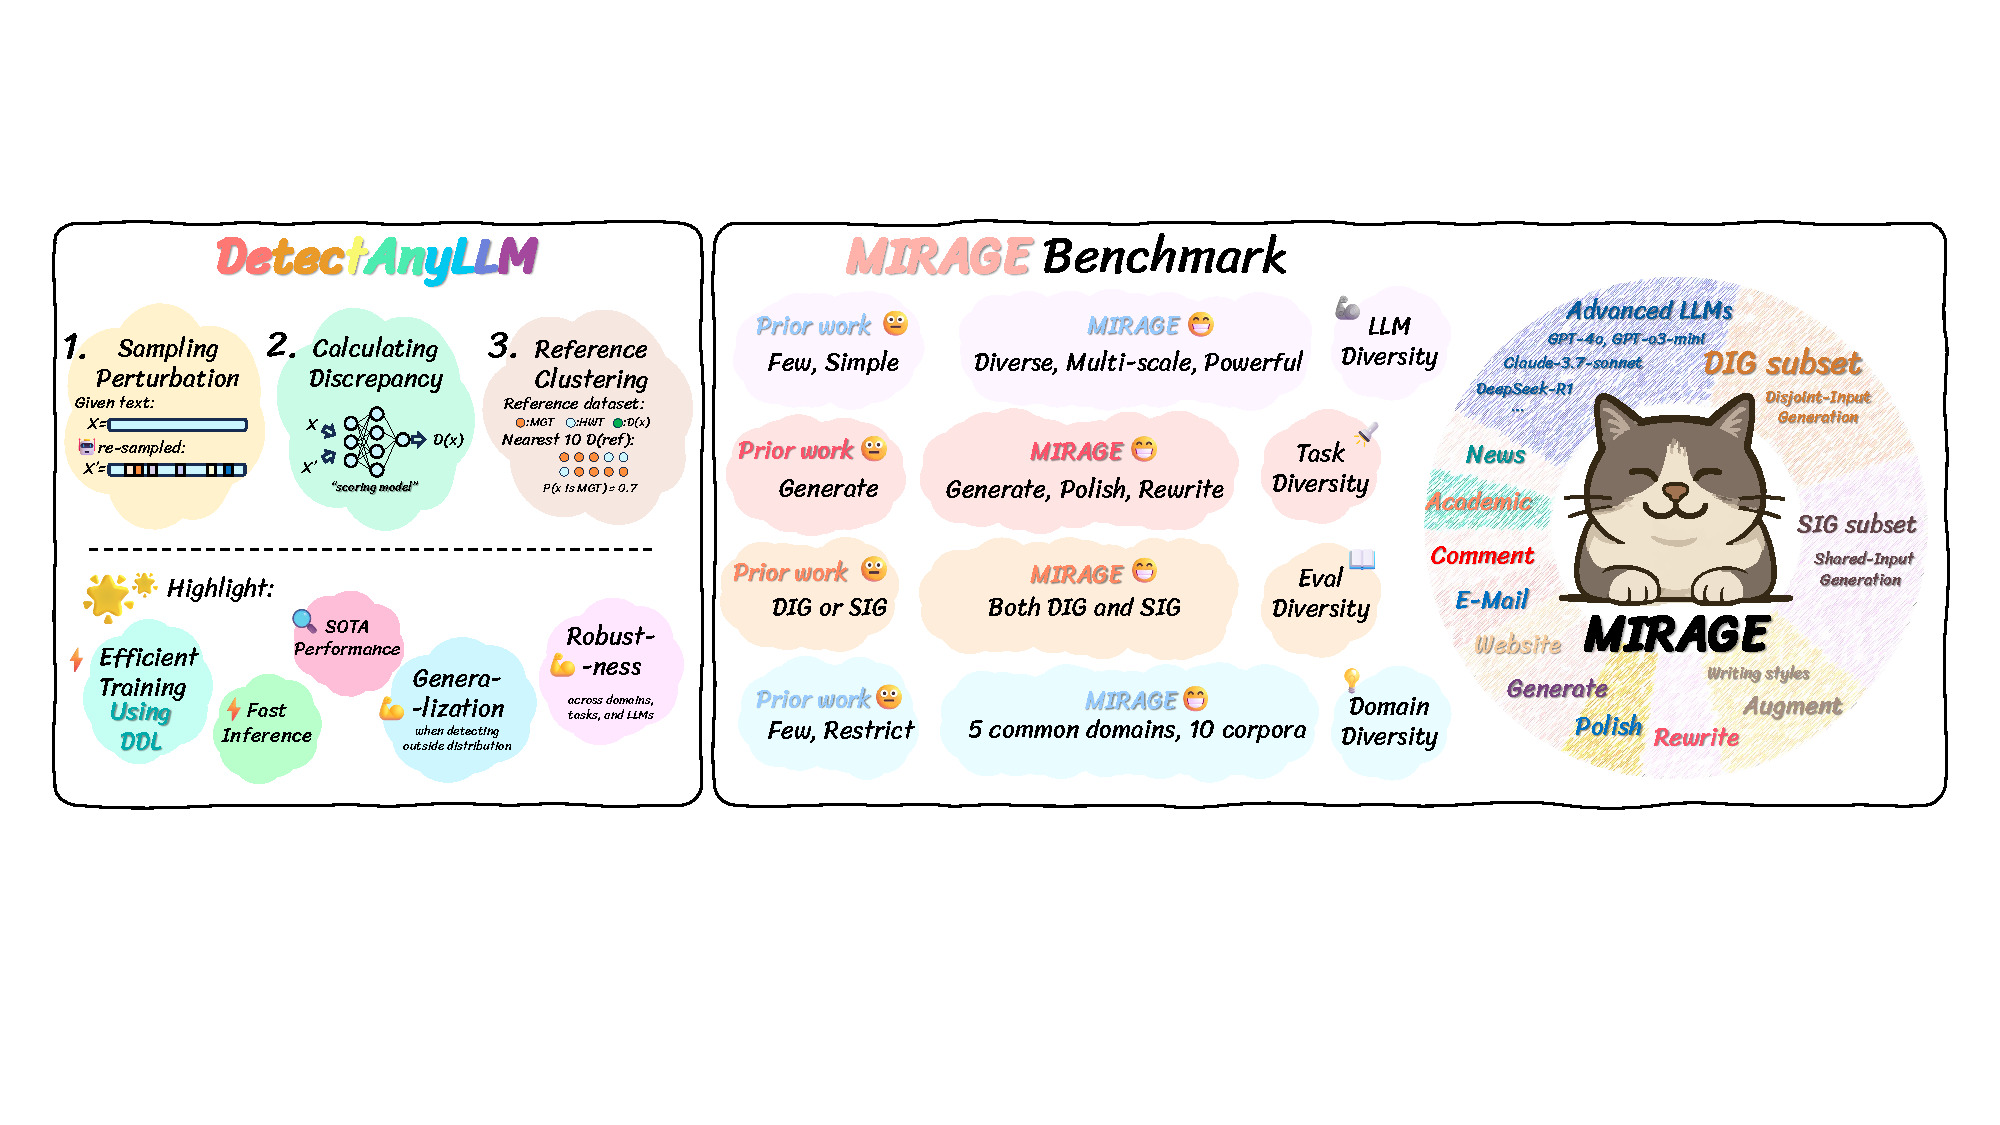
\includegraphics[width=\textwidth]{fig/teaser.pdf}
  \caption{Left: Our DetectAnyLLM achieves high efficiency, strong robustness, and impressive generalization through a three-step process: \textit{sampling perturbation}, \textit{calculating discrepancy}, and \textit{reference clustering}. Right: Our MIRAGE benchmark emphasizes diversity across domains, tasks, evaluation scenarios, and source LLMs, enabling comprehensive and robust evaluation.}
  \Description{Overview of our work. }
  \label{fig:teaser}
\end{teaserfigure}

\maketitle

\section{Introduction}
% \begin{figure*}[t]
%     \centering
%     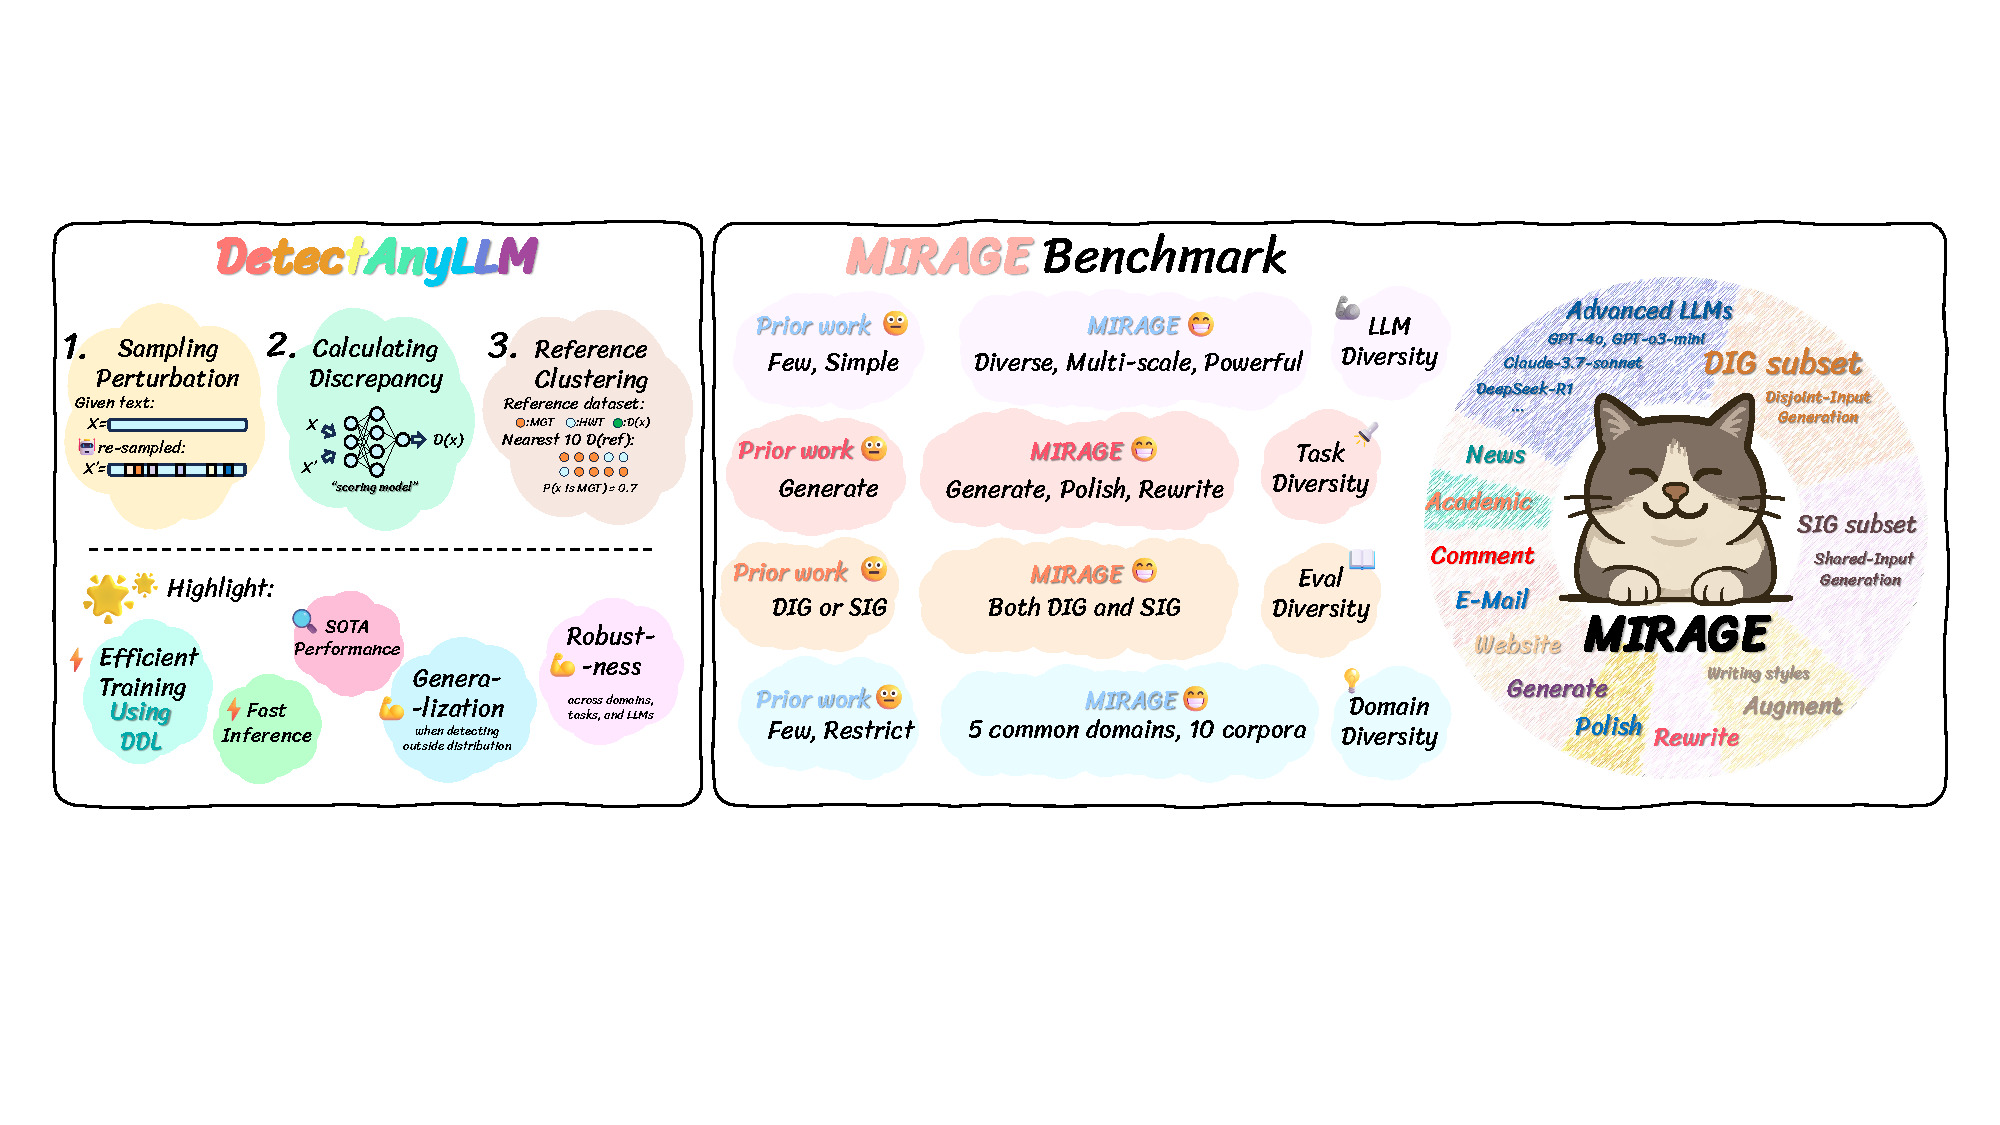
\includegraphics[width=\linewidth]{fig/teaser.pdf}
%     \caption{Overview of our work.}
%     \Description{Simple look of our work.}
%     \label{fig:main}
% \end{figure*}
%\noindent \textbf{Why detect?}
Advanced generative \textit{Large Language Models (LLMs)}~\cite{gpt4, gpt4o, deepseekr1, deepseekv3, gpto1} can easily generate text nearly indistinguishable from human writing~\cite{indistinguish_1, indistinguish_2}.
%
If such technology is misused, it could pose serious risks to society.
%
% For example, 
% in academic research, the inability to distinguish between human-authored papers and LLM-generated content could undermine the credibility of scholarly work. 
%
% Similarly, 
% if we cannot determine whether news reports are written by human journalists or fabricated by LLMs~\cite{fakenews}, the integrity of information and public trust in the media could be significantly compromised. %\lichongyi{this sentence can be removed if we do not have enough space.}
%\noindent \textbf{Task define}
In response to such concern, the task of \textit{Machine-Generated Text Detection (MGTD)} has emerged~\cite{logrank, entropy, likelihood}.
%
MGTD is a binary classification task designed to distinguish whether a given text is completely written by humans or generated (or revised) by a machine.
%
Note that, in this study, MGTD includes detection of both \textit{Machine-Generated Text (MGT)} and \textit{Machine-Revised Text (MRT)}, where MRT refers to text that has been polished or rewritten by a model based on an original \textit{Human-Written Text (HWT)}.


%\noindent \textbf{Baseline? Theory?}
As MGT and MRT have distinct token probability distributions compared to HWT, several MGTD methods have been proposed~\cite{logrank, likelihood, entropy, detectgpt, fastdetectgpt}. 
%
Most of them leverage pre-trained language models, referred to as \textit{scoring models}, to estimate the token probabilities of a given text and compute classification metrics for distinguishing between human-written and machine-generated content.


Existing MGTD methods can be further categorized into zero-shot detection methods~\cite{entropy, lrrandnpr, detectgpt, fastdetectgpt, hart} and training-based detection methods~\cite{logrank, imbd}.
%
%\todel{The performance of zero-shot methods is often constrained, as they rely heavily on the original output distribution of the scoring model~\cite{glimpse}. However, scoring models are usually small-scale LLMs (e.g. GPT-Neo-2.7B~\cite{gpt-neo}), which have limited knowledge and simpler output patterns compared to large-scale models. As a result, they struggle to effectively detect text outside of their original distributions, causing the performance of zero-shot detection to be heavily dependent on the capabilities of the scoring model itself.}
%
Zero-shot methods typically rely on the original output distributions of pre-trained scoring models~\cite{glimpse}, which constrains their performance. This limitation arises because scoring models are often relatively small-scale language models (e.g., GPT-Neo-2.7B~\cite{gpt-neo}), which possess restricted knowledge and comparatively simplistic output patterns. However, detection often happens with texts that deviate from their inherent distribution, making it difficult for these methods to realize reliable detection.
%
Training-based methods use \textit{supervised fine-tuned (SFT)}~\cite{sft, logrank} or \textit{preference learning}~\cite{orpo, dpo, imbd} to align the scoring model's output distribution with that of a specific model.
%
While this approach improves detection performance for that specific model, it often causes the scoring model to overfit the training data~\cite{overfit, outdomain}. As a result, the detector's ability to generalize and remain robust when detecting outside the training distribution is compromised~\cite{fastdetectgpt, survey_necessity_methods_futuredirect, survey_science}. %\lichongyi{why?}

%\noindent \textbf{Motivation}
In this study, we find that the key to improve the generalization and robustness of the detector lies in training the scoring model to capture more intrinsic differences between MGT and HWT, rather than merely optimizing the token probability distributions.
%
Furthermore, we observe that even the most advanced training-based methods~\cite{imbd, pawn} primarily fine-tune the scoring model to align its output distribution with that of the target model they aim to detect, rather than directly training the scoring model as a dedicated detector, which may hinder performance on the MGTD task..

Building on such observations, we propose a novel optimization strategy, \textbf{Direct Discrepancy Learning (DDL)}, that enables the model to \textbf{learn to be a detector rather than another language model} by directly optimizing the scoring model with its output classification metric.
%
DDL aims to free the scoring model from the constraints of its original language model identity so that it can focus on learning the intrinsic knowledge of MGT detection rather than merely fitting the distribution of the training data. 

Furthermore, as the fusion of prior approaches~\cite{fastdetectgpt, imbd} and DDL, we propose \textbf{DetectAnyLLM}, a unified MGTD framework.
%
DetectAnyLLM achieves efficient and robust detection through three steps comprising \textit{re-sampling}, \textit{discrepancy calculation}, and \textit{reference clustering}.
%
Such a framework distills the core insights of existing methods~\cite{detectgpt, fastdetectgpt} while leveraging DDL to enhance the model’s generalization capabilities and improve detection robustness.
%\lichongyi{we need a figure to show the performance improvement of our strategy. We can put it on the top right of the first page.}
\begin{table*}[htbp]
    \centering
    \caption{Comparison between MIRAGE and existing MGTD benchmark datasets. ``Size" is the capacity of the test set. ``SIG" denotes Shared-Input Generation and ``DIG" denotes Disjoint-Input Generation. ``Commercial" refers to the use of frontier proprietary LLMs (e.g., GPT-4o). MIRAGE is the most diverse benchmark in terms of domain, tasks, and source LLMs. MIRAGE leverages powerful commercial LLMs to generate and revise text, increasing the difficulty of detection and the realism of evaluation, enabling a more faithful evaluation of detector robustness. Furthermore, MIRAGE introduces a novel dual-scenario evaluation strategy —DIG and SIG— allowing more comprehensive assessment of both accuracy and generalization capacity.}
    \renewcommand{\arraystretch}{1.25}
    \resizebox{\linewidth}{!}{
    \begin{tabular}{l|ccc|c|ccc|ccc}
    \hline

    \hline

    \hline
    &\multicolumn{3}{c|}{\textbf{Data Statistic}}&\multicolumn{1}{c|}{\textbf{LLMs}}&\multicolumn{3}{c|}{\textbf{MGT Tasks}}&\multicolumn{3}{c}{\textbf{Other}}\\
    \textbf{Benchmark}& Size & Domain Coverage & Corpus & Commercial & Generate & Polish & Rewrite & Aug. & SIG & DIG\\
    \hline
    TuringBench~\cite{turingbench}& 40K & News & 3 & \wrong & \correct & \wrong & \wrong & \wrong & \wrong & \correct\\
    HC3~\cite{hc3}& 85K & QA/Comment/Academic & 5 & 1  & \correct & \wrong & \wrong & \wrong & - & - \\
    M4~\cite{m4bench}& 24.5K & QA/Comment/Academic/News & 11 & 2 & \correct & \wrong & \wrong & \correct & \correct & \wrong\\
    MAGE~\cite{mage}& 29K & QA/Comment/News/Academic/Story & 10 & 3 & \correct & \wrong & \wrong & \correct & \correct & \wrong \\
    RAID~\cite{raid}& 628.7K & News/Academic/Comment/Literature& 11& 3 & \correct & \wrong & \correct & \correct & \correct & \wrong\\
    DetectRL~\cite{detectrl}&134.4K& Academic/Comment & 4 & 2&\correct&\wrong&\correct&\correct&\correct&\wrong \\
    HART~\cite{hart}&16K& News/Literature/Academic& 4 & 4 & \correct & \correct &\correct &\correct & \wrong & \correct \\    
    \rowcolor[HTML]{fff5f4}
    \textbf{MIRAGE (ours)}&93.8K &Academic/Comment/Email/News/Website & 10 & 13 & \correct & \correct & \correct & \correct & \correct & \correct \\
    \hline

    \hline

    \hline
    \end{tabular}
    }
    \label{tab:benchmarks}
\end{table*}

\begin{figure}[t]
    \centering
    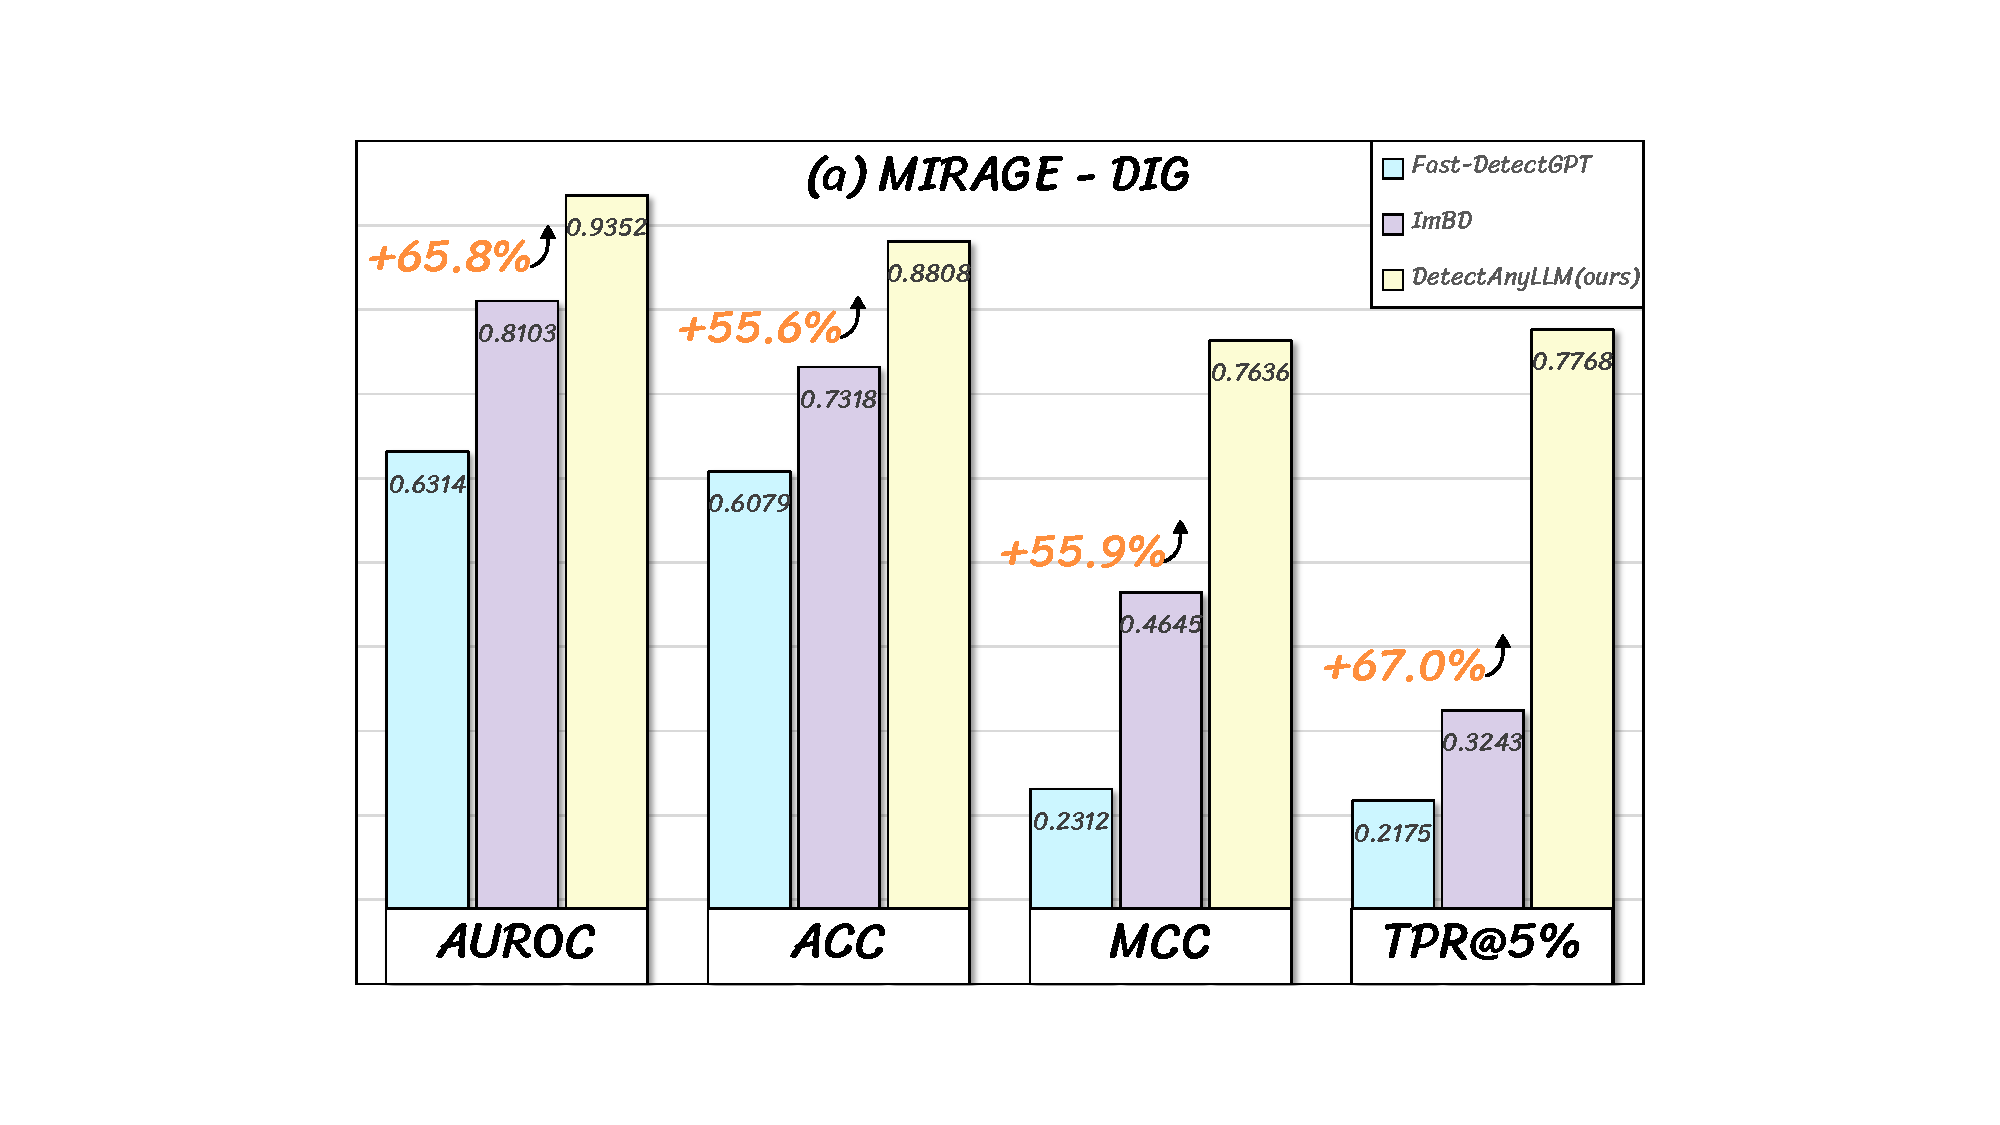
\includegraphics[width=0.985\linewidth]{fig/performance_comparison.pdf}
    \caption{Performance on MIRAGE-DIG for DetectAnyLLM and state-of-the-art methods, including Fast-DetectGPT~\cite{fastdetectgpt} and ImBD~\cite{imbd}. Improvement: $(new-old)/(1.0-old)$.}
    \Description{Performance Comparison on MIRAGE. The DIG subset reflects abilities across domains, and the SIG subset reflects abilities across generators.}
    \label{fig:performance_comparison}
\end{figure}

%\noindent \textbf{Benchmark}
In addition, despite the emergence of various MGTD studies, there remains a lack of comprehensive benchmarks~\cite{survey_necessity_methods_futuredirect}.
%
Existing benchmarks~\cite{mage, mgtbench, detectrl} suffer from several significant deficiencies: \textbf{1) Limited focus on MRT:} Most benchmark datasets, such as MGTBench~\cite{mgtbench}, focus solely on MGT while neglecting the detection of MRT. \textbf{2) Narrow range of source LLMs:} Most benchmarks rely on small-scale, open-source models, whereas real-world applications often involve advanced, closed-source LLMs such as GPT-4o~\cite{gpt4o} and DeepSeek-R1~\cite{deepseekr1}.  \textbf{3) Restricted domain coverage:} Benchmarks such as HC3~\cite{hc3} typically sample text from only one or a few domains, neglecting the domain sensitivity of machine-generated text.
%
These deficiencies highlight a significant gap between existing benchmark datasets and real-world applications, indicating that current benchmarks fail to comprehensively and objectively reflect real-world detection challenges.


Although some recent studies~\cite{survey_necessity_methods_futuredirect, hart} have recognized this issue, their datasets remain insufficiently comprehensive.
%
To facilitate further research,  we construct \textbf{MIRAGE}, the largest multi-task MGTD benchmark that provides the richest variety of commercial LLMs and the most comprehensive text domains in MGTD research.
%
As shown in ~\Cref{tab:benchmarks}, MIRAGE samples text from \textbf{10 corpora} in \textbf{5 common domains}, and uses \textbf{17 advanced mainstream LLMs} for text generation or revision, creating over \textbf{93K HWT-MGT pairs}.
%
MIRAGE establishes a more realistic and reliable evaluation standard, bridging the gap between research and real-world applications.


Though existing detection methods have demonstrated seemingly outstanding performance (AUC > 0.9) on previous benchmarks~\cite{imbd, detectrl}, they exhibit significant weaknesses when evaluated on MIRAGE, as ~\Cref{fig:performance_comparison} shown.
%
This reveals the generalization and robustness of prior methods require substantial improvement. 
%
In contrast, DetectAnyLLM still performs well, achieving an average of \red{0.9352} AUROC and \red{0.7636} MCC on the MIRAGE-DIG subset.
%
Such performance powerfully demonstrates the effectness and superior generalization of DDL.


Our contributions can be summarized into the following points:


\begin{itemize}[leftmargin=*]
    \item We propose a novel optimization strategy for MGTD, termed \textbf{Direct Discrepancy Learning (DDL)}, enabling the model to
    %function explicitly as a detector rather than another language model, thereby 
    directly acquire task-oriented knowledge. DDL greatly improve detector's generalization and robustness with fewer computational resources and no additional training data.
    \item We construct a comprehensive benchmark dataset for MGTD, named \textbf{MIRAGE}, which covers the most diverse text domains, MGT tasks, and source LLMs. MIRAGE novelly focuses on using commercial LLMs to generate data, enhancing the realism and practical relevance of evaluation.
    %Extensive experiments on MIRAGE reveal that existing MGTD methods heavily fall short in performance across various challenging scenarios.
    \item We present \textbf{DetectAnyLLM} framework, unifying prior works and DDL. DetectAnyLLM achieve \textbf{50\%-70\%} performance improvement over previous state-of-the-art methods, realizing a generalizable and robust detection across domains and models.
    %—demonstrating the effectiveness and efficiency of DDL.
\end{itemize}

% \noindent \textbf{Contribution}
\section{Related Work}
\subsection{Zero-shot Detector}
Previous MGTD research emphasized zero-shot detection due to concerns about overfitting during training~\cite{outdomain, overfit}. 
%
Early methods like GLTR~\cite{entropy} leveraged text entropy to detect machine content, while others used likelihood- or ranking-based approaches~\cite{likelihood, logrank}.
%
Recently, Detect-GPT~\cite{detectgpt} has been proposed, which distinguishes MGT from HWT using \textit{perturbation}, \textit{scoring}, and \textit{probability curvature estimation}, providing a novel view for MGTD.
%
%
DetectLLM~\cite{lrrandnpr} further improves the performance by adding Log-Rank Score.
%
Fast-DetectGPT~\cite{fastdetectgpt} improves the perturbation step, significantly accelerating the detection process without sacrificing performance.
%
Despite progress, zero-shot methods remain constrained by their dependence on the scoring model’s output distribution, as shown by Glimpse~\cite{glimpse}, which demonstrated performance improvement through stronger scoring models.


\subsection{Training-based Detector}
The training-based detector fine-tunes the scoring model on specific training data.
%
An early representative work is RoBERTa-OpenAI-Detector~\cite{likelihood}, the researchers fine-tune RoBERTa~\cite{roberta} models using GPT-2~\cite{gpt2}-generated data, performing well on detecting GPT-generated text.
%
RADAR~\cite{radar} incorporates adversarial training~\cite{gan} to enhance MGTD robustness and uses PPO~\cite{ppo} to optimize the generator, improving the generator-generated-text's similarity to HWT. 
%
More recently, ImBD~\cite{imbd} utilizes DPO~\cite{dpo} to optimize the scoring model in Fast-DetectGPT~\cite{fastdetectgpt}, aiming to help the scoring model better capture the style features of the training data.

Despite these advancements, most methods simply focus on training the scoring model to approximate the source model’s distribution rather than developing a dedicated MGTD detector. 
%
This introduces constraints to the scoring model during training, which are detrimental to the MGTD task.
%
By freeing the scoring model from its language model's identity constraint, we enable it to \textbf{learn to be a detector rather than another language model}, thereby enhancing its generalization ability.


\subsection{MGTD Benchmark}
Early benchmarks like Turingbench~\cite{turingbench} focused on news articles generated by neural models, while the emergence of ChatGPT~\cite{instructGPT} shifted attention to LLM-generated text, exemplified by MGTBench\cite{mgtbench} and HC3~\cite{hc3}. 
%
Later efforts such as MAGE~\cite{mage}, MULTITuDE~\cite{multitude}, and M4~\cite{m4bench} explored open-domain and multilingual detection.
%
RAID~\cite{raid} novelly introduced decoding strategy considerations to strengthen evaluation robustness, while DetectRL~\cite{detectrl} examined vulnerabilities from a writing-attack perspective.
%
However, most of these benchmarks rely on open-source models (indicating limited variousity) and focus mainly on MGT, overlooking more common real-world applications involving MRT, thus limits their applicability to real-world contexts.

HART~\cite{hart} marked progress by incorporating both MGT and MRT using six advanced LLMs (only four commercial LLMs), but it remains limited in generator diversity and domain scope.
%
In this study, we scale up the number of generators to 17, where 13 are commercial LLMs and 4 are advanced open-source LLms, covering nearly all major LLMs used in real-world applications.
%
Moreover, we sample HWT from five distinct domains and generate both MGT and MRT, ensuring a more comprehensive and representative evaluation.
%
To advance MGTD research and enable fairer comparisons, we advocate for the adoption of a unified benchmark to ensure consistency in evaluation standards. We hope that our benchmark will serve as a valuable step toward achieving this goal.
\section{DetectAnyLLM Framework}
DetectAnyLLM builds upon Fast-DetectGPT~\cite{fastdetectgpt}, which determines whether a text is MGT by measuring the log-probability discrepancy between the original text and its perturbed variants~\cite{detectgpt}.
%
This method involves three key steps: \textit{1) re-sampling the given text}, \textit{2) computing the discrepancy between original text and re-sampled text}, and \textit{3) making a decision using the discrepancy}.
%
In \Cref{3.1}, we describe how the log-probability discrepancy is calculated.
%
Next, in \Cref{3.2}, we explain the motivation behind our improvements to this detection process, along with the specific designs we introduce.
%
Finally, in \Cref{3.3}, we detail how discrepancy is ultimately used for MGTD within our proposed framework.

\subsection{Preliminary}\label{3.1}


\noindent \textbf{Basic Hypothesis. }
%Our work shares a same hypothesis with ~\cite{fastdetectgpt} and ~\cite{detectgpt}, that is, 
Machine-generated text tends to consist of high-probability tokens at each position, whereas human-written text has greater variability.
%
Although sampling strategies like top-k and top-p introduce some randomness, LLMs still generally select tokens with relatively high probabilities.
%
Thus, features in the probability distribution of tokens can serve as useful cues for distinguishing machine-generated text from human-written.


\noindent \textbf{Probability Discrepancy. }
Given a text $x$ and a scoring model $f_\theta$, when using another language model $q_\phi$ to produce perturbations, the \textit{probability discrepancy} (i.e., probability curvature)~\cite{detectgpt} can be expressed as:
\begin{equation}
    d(x, f_\theta, q_\phi) = \log f_\theta(x) - \mathbb E_{\tilde{x} \sim q_\phi(\cdot|x)}[\log f_\theta(\tilde{x})],
    \label{3.1.1}
\end{equation}
where $\tilde{x}$ is the perturbed version of $x$ by $q_\phi$.

% Based on the hypothesis, machine-generated text $x_m$ tends to have high log-probability, whereas its perturbed version $\tilde{x_m}$ shows a lower log-probability.
% %
% In contrast, human-written text $x_h$ generally has a lower log-probability.
% %
% When perturbed, $\tilde{x_h}$ tends to show an increase in log-probability, as the perturbation process replaces words in $x_h$ with higher-likelihood alternatives according to the model.
% %
% Thus, we expect to achieve:
% \begin{equation}
%     d(x_m, f_\theta, q_\phi) > d(x_h, f_\theta, q_\phi).
%     %\tag{3.1.2}
%     \label{3.1.2}
% \end{equation}
% %
% This inequality forms the basis of MGTD~\cite{detectgpt, fastdetectgpt, imbd}.

% When calculating this discrepancy, achieving $f_\theta$ is straightforward, allowing $\log f_\theta(x)$ to be efficiently computed using a Markov chain.
% %
% However, estimating the expectation of the log-probability of $\tilde{x}$ is more complex.
% %
% DetectGPT~\cite{detectgpt} addresses the estimation by generating many perturbations $\tilde{x}$ and approximating the expectation using the mean log-probability of these samples.
% %
% Since log-probabilities are computed using a Markov chain, even a small perturbation requires recalculating the entire chain, thus DetectGPT~\cite{detectgpt} has a high computational complexity.
% While effective, this approach requires computing log-probabilities for numerous perturbations, making it computationally expensive and less practical for real-world applications.

When calculating this discrepancy, achieving $f_\theta$ is straightforward, allowing $\log f_\theta(x)$ to be efficiently computed.
%
However, since the log-probabilities are computed using Markov-Chain, even a small perturbation requires recalculating the entire chain.
%
Thus, estimating the expectation of the log-probability of $\tilde{x}$ is complex.

\noindent \textbf{Fast-DetectGPT. }~\cite{fastdetectgpt} introduced \textit{conditional probability}, which provides a biased yet computationally efficient estimation of the original probability:
\begin{equation}
    f_\theta(\tilde{x}) = \prod_{i}f_\theta(\tilde{x}_i|\tilde{x}_{<i}) \sim \prod_{i}f_\theta(\tilde{x}_i|x_{<i}) = f_\theta(\tilde{x}|x).
    %\tag{3.1.3}
    \label{3.1.3}
\end{equation}
%
By introducing Eq.~\eqref{3.1.3}, the probability discrepancy in Eq.~\eqref{3.1.1} can be further reformulated to the\textit{conditional probability discrepancy}:
\begin{equation}
    d_c(x, f_\theta, q_\phi) = \frac{\log f_\theta(x|x) - \tilde{\mu}}{\tilde{\sigma}},
    %\tag{3.1.4}
    \label{3.1.4}
\end{equation}
where
\begin{equation}
\begin{aligned}
    \tilde{\mu} &= \mathbb E_{\tilde{x}\sim q_\phi(\tilde{x}|x)}[\log f_\theta (\tilde{x}|x)],\\
    \tilde{\sigma}^2 &= \mathbb E_{\tilde{x}\sim q_\phi(\tilde{x}|x)}[\log f_\theta (\tilde{x}|x) - \tilde{\mu}^2].
\end{aligned}
%\tag{3.1.5}
\label{3.1.5}
\end{equation}
% In Eq.~\eqref{3.1.4},  $\log f_\theta(x|x)$ is a unbiased estimation of $\log f_\theta(x)$, which is the first item of Eq.~\eqref{3.1.1}.
% %
% In addition,  $\tilde{\mu}$ is a biased estimation of $\mathbb E_{\tilde{x}\sim q_\phi(\cdot|x)}[\log f_\theta(\tilde{x})]$, representing the second term in Eq.~\eqref{3.1.1}.
%
Noticing that a normalization item $\tilde{\sigma}$ is added into the discrepancy function, we further explore how the $\tilde{\sigma}$ affects performance in ~\Cref{ablation_on_sigma}.
%
% This normalization enhances detection accuracy and ensures that discrepancy distributions remain comparable across different models and datasets, thus improves robustness in real-world applications.
%
Eq.~\eqref{3.1.4} forms the discrepancy we use in our study.

Based on the hypothesis, machine-generated text $x_m$ tends to have a high log-probability, whereas its perturbed version $\tilde{x_m}$ shows a lower log-probability.
%
In contrast, human-written text $x_h$ generally has a lower log-probability.
%
When perturbed, $\tilde{x_h}$ tends to show an increase in log-probability, as the perturbation process replaces words in $x_h$ with higher-likelihood alternatives according to the model.
%
Thus, we expect to achieve:
\begin{equation}
    d(x_m, f_\theta, q_\phi) > d(x_h, f_\theta, q_\phi).
    %\tag{3.1.2}
    \label{3.1.2}
\end{equation}
%
This inequality forms the basis of MGTD~\cite{detectgpt, fastdetectgpt, imbd}.

% Observing Eq.~\eqref{3.1.4}, we note that that  the discrepancy $d$ increases when $f_\theta$ assigns a higher probability to $x$ than to its perturbed version $\tilde{x}$.
% %
% Based on our \lichongyi{our?} hypothesis, since the scoring model $f_\theta$ prefers high-probability tokens at each position, detection performance can be improved by increasing the probability discrepancy between MGT and HWT within the model’s output distribution.
% %
% To achieve this, \cite{imbd} introduced \textit{Direct Preference Optimization (DPO)}~\cite{dpo} and believed that utilizing DPO to optimize instead of using MSE, enables the model to learn stylistic features more effectively, thereby enhancing the robustness of the detector.
% %
% However, we suggest that DPO can only help the scoring model learn to be another LLM rather than a detector. This creates a gap in the model’s ability to handle MGTD effectively
% \lichongyi{preliminary is overlength. Some content can be removed to Introduction. Moreover, we cannot copy the content from the original paper. In Preliminary, just present the basic idea and workflow, even the limitations.}

\begin{figure}[t]
    \centering
    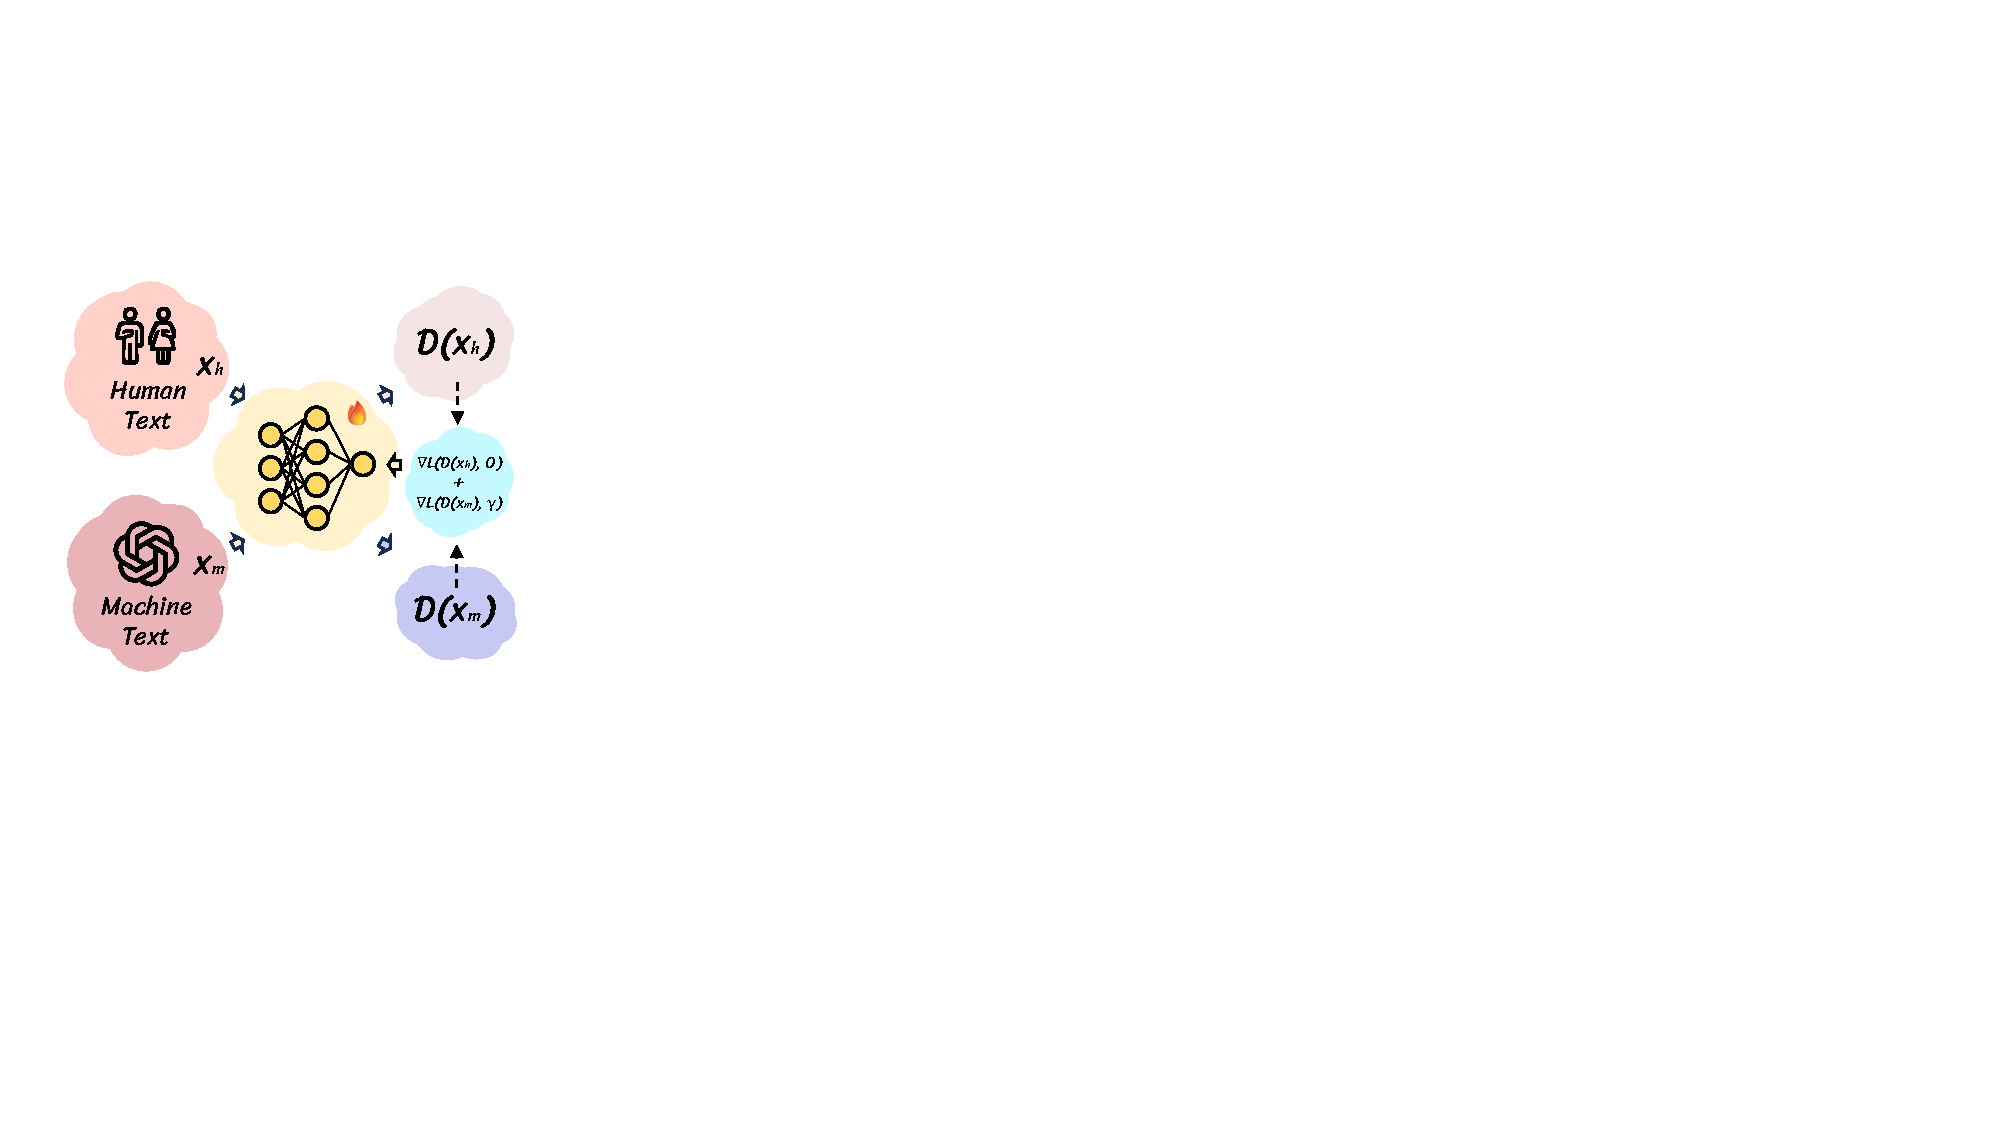
\includegraphics[width=0.65\linewidth]{fig/ddl.pdf}
    \caption{Overview of Direct Discrepancy Learning. The scoring model receives paired HWT-MGT data and computes the discrepancy for each. We optimize it to minimize the HWT's discrepancy while maximizing the MGT's.}
    \Description{Overview of Direct Discrepancy Learning. }
    \label{fig:ddl}
\end{figure}

\subsection{Optimizing by Direct Discrepancy Learning}\label{3.2}
As shown in Eq.~\eqref{3.1.4} and Eq.~\eqref{3.1.2}, the key to enhance the detector's performance is to increase the scoring model's probability distribution discrepancy between MGT and HWT.

While ImBD~\cite{imbd} has achieved significant performance gains by incorporating \textit{Direct Preference Optimization (DPO)}~\cite{dpo} to optimize the scoring model, we argue that DPO is not the optimal optimization method for the MGTD task.
%
This is because DPO implicitly aligns the scoring model with the preferences of another language model, rather than directly optimizing the scoring model to classify MGT and HWT. 
%
Moreover, such alignment could mislead the scoring model from learning the MGTD-oriented knowledge, thus do harm to the detector's generalization performance.


\noindent \textbf{DPO.}
~\cite{dpo} is derived from the optimization objective of \textit{Proximal Policy Optimization (PPO)}~\cite{ppo}, which is:
\begin{equation}
    \mathop{max}_\theta \mathbb{E}_{x\sim f_\theta(x)}[r(x)] - \beta\mathbb{D}_{KL}[f_\theta(x) \mid \mid f_{ref}(x)],
    \label{3.2.1}
\end{equation}
where $x$ is a text sampled from the scoring model $f_\theta$'s distribution, and $r$ is a reward function that can judge whether this sample is bad or good.
%
By analyzing and re-parameterizing this optimization objective, we can obtain DPO's optimization objective:
\begin{equation}
    \mathop{max}_\theta \mathbb{E}_{x_m, x_h \sim \mathop{D}}[\log \sigma(\beta\log\frac{f_\theta(x_m)}{f_{ref}(x_m)}-\beta\log\frac{f_\theta(x_h)}{f_{ref}(x_h)})],
    \label{3.2.6}
\end{equation}
where $x_m$ denotes MGT and $x_h$ stands for HWT.
%
$f_{ref}$ is a reference model, usually the original $f_\theta$.
%
The detailed derivation process will be presented in the supplementary material.

\noindent \textbf{Redundant KL-regularization. }\label{redundant KL-regularization}
The KL-regularization between $f_\theta$ and $f_{ref}$ is explicitly added to the optimization objective in PPO~\cite{ppo}, and its weight is adjusted via $\beta$, as shown in Eq. \eqref{3.2.1}.
%
While in DPO~\cite{dpo}, as Eq. 
\eqref{3.2.6} shown, such regularization is implicitly embedded in the optimization objective, and its strength can also be adjusted by $\beta$.
%
ImBD~\cite{imbd} directly adopts Eq.\eqref{3.2.6} as its loss function and leverages paired MGT-HWT data to optimize the scoring model $f_\theta$.
%
The KL-regularization forces the scoring model to retain its internal knowledge while learning preferences.

\textit{This leads us to question: for the MGTD task, what is the significance of retaining the original knowledge of the scoring model during training?}

Since we have already collected data and introduced training, our direct objective should be enable the scoring model to better learn the features of the source model from the training data.
%
While fundamentally, we hope that the training process will teach the scoring model how to become a detector.
%
However, the KL-regularization drastically shifts this objective: from learning the intrinsic knowledge of the MGTD task to aligning the scoring model with the distribution of training data.
%
Thus shifts the training process from learn a detector to learn a language model.
%
Such an optimization objective fails to directly reflect task requirements, thereby limiting the detector's performance potential.

%Experiments on the impact of the KL-strength $\beta$ on ImBD~\cite{imbd} is provided in the Supplementary Material.

\noindent \textbf{Direct Discrepancy Learning. }
We observed that by simply removing the KL-regularization from the optimization objective, the robustness and generalization of the model can be significantly improved. Thus, the optimization goal can be re-written as:
\begin{equation}
    \mathop{max}_{\theta} \mathbb{E}_{x\sim \mathop{D}}[r(x)].
    %\tag{3.3.1}
    \label{3.3.1}
\end{equation}
Furthermore, we utilize a simple reward function $r(x)$, defined as:
\begin{equation}
    r(x) = \begin{cases}
    -\Vert \gamma - d_c(x, f_\theta, q_\phi) \Vert_1, & \text{when $x$ is $x_m$,}\\
    -\Vert d_c(x, f_\theta, q_\phi) \Vert_1, & \text{when $x$ is $x_h$.}
    \end{cases}
    %\tag{3.3.2}
    \label{3.3.2}
\end{equation}
where $\gamma$ is an hyper-parameter.
%
This reward function is designed based on the conclusions discussed in Section~\ref{3.1}, that is the discrepancy of human-written text $x_h$ tends to be low (close to 0) while the discrepancy of machine-generated text $x_m$ tends to be positive.
%
The parameter $\gamma$ is introduced to control how positive the discrepancy of $x_m$ should be.
%
In our experiment, $\gamma$ is arbitrarily chosen.
%
As ~\Cref{tab:ablation_gamma}, experiment on the impact of the value of $\gamma$, shown that the model's performance is not particularly sensitive to this choice, indicating a level of robustness to variations in $\gamma$. 
%
In practice, our input consists of paired HWT-MGT data. We set $q_\phi = f_\theta$ following the ImBD~\cite{imbd}'s setting, which allows us to use the scoring model’s output for optimization: 
\begin{equation}
    \mathop{min}_\theta \mathbb{E}_{x_m, x_h \sim \mathop{D}}(\Vert d_c(x_h, f_\theta, f_\theta)\Vert_1 + \Vert \gamma - d_c(x_m, f_\theta, f_\theta)\Vert_1).
   % \tag{3.3.3}
    \label{3.3.3}
\end{equation}
We call this optimization method as \textit{Direct Discrepancy Learning (DDL)}, as it helps the scoring model directly learning the discrepancy between MGT and HWT.

%\noindent \textbf{Analysis. }
By removing the KL-regularization, the scoring model can essentially forget its identity as a language model and instead focus on learning task-oriented knowledge, which is critical for the MGTD task.
%
Furthermore, we introduce a reward function based on the discrepancy $d_c$, which incorporates a task-oriented prior, and thus can further help the scoring model learn the knowledge of MGTD.
%
Specifically, $d_c$ for HWT approaches $0$, while $d_c$ for MGT is positive.


\subsection{Detecting by Reference Clustering}\label{3.3}
We use \textit{Reference Clustering} to achieve the transition from $d_c(x)$ to $p_{m}(x)$.
%
Specifically, this algorithm is designed to estimate the probability of a given value belonging to a specific distribution, consisting of: \textit{data aggregation} and \textit{probability estimation}.

\noindent \textbf{Data Aggregation. }
We first collect a certain number of MGT texts as the MGT reference dataset $M$, and an approximately equal number of HWT texts as the HWT reference dataset $H$.
%
Then, we employ the scoring model $f_\theta$, which will be used for detection, to respectively compute the conditional probability discrepancy $d_c$ for each text in $M$ and $H$.
%
Thereby , we can obtain the conditional probability discrepancy distribution $D_m$ and $D_h$ of the texts in $M$ and $H$ under scored by $f_\theta$.


\noindent \textbf{Probability Estimation. }
We select the value in $M\cup H$ that is $k_{th}$ closest to the target value $d_c(x)$ as the search window $\delta$:
\begin{equation}
    \delta = sorted(\{\Vert d_c(x_{ref}) - d_c(x)\Vert_1 \mid x_{ref}\in M \cup H\})[k],
    \label{3.3.4}
\end{equation}
where $k$ is a hyper-parameter that should be determined by the size of reference dataset.
%
For a larger reference dataset, a larger $k$ is better as it can provide higher precision of $p_{m}(x)$.

Then, we count the number of MGT texts and HWT texts within the window range:
\begin{equation}
    \begin{aligned}
        cnt_m = \sum_{d\in D_m}I(d_c(x) - \delta < d < d_c(x) + \delta),\\
        cnt_h = \sum_{d\in D_h}I(d_c(x) - \delta < d < d_c(x) + \delta).
    \end{aligned}
    \label{3.3.5}
\end{equation}
Finally, we estimate the probability that text $x$ belongs to MGT using the local statistical ratio:
\begin{equation}
    p_m(x) = \frac{cnt_m}{cnt_m + cnt_h}.
    \label{3.3.6}
\end{equation}

Since the window $\delta$ is adaptively determined by the data distribution, this method can maintain stability under different data densities, thereby improving the robustness of real-world MGTD.

\begin{figure*}
    \centering
    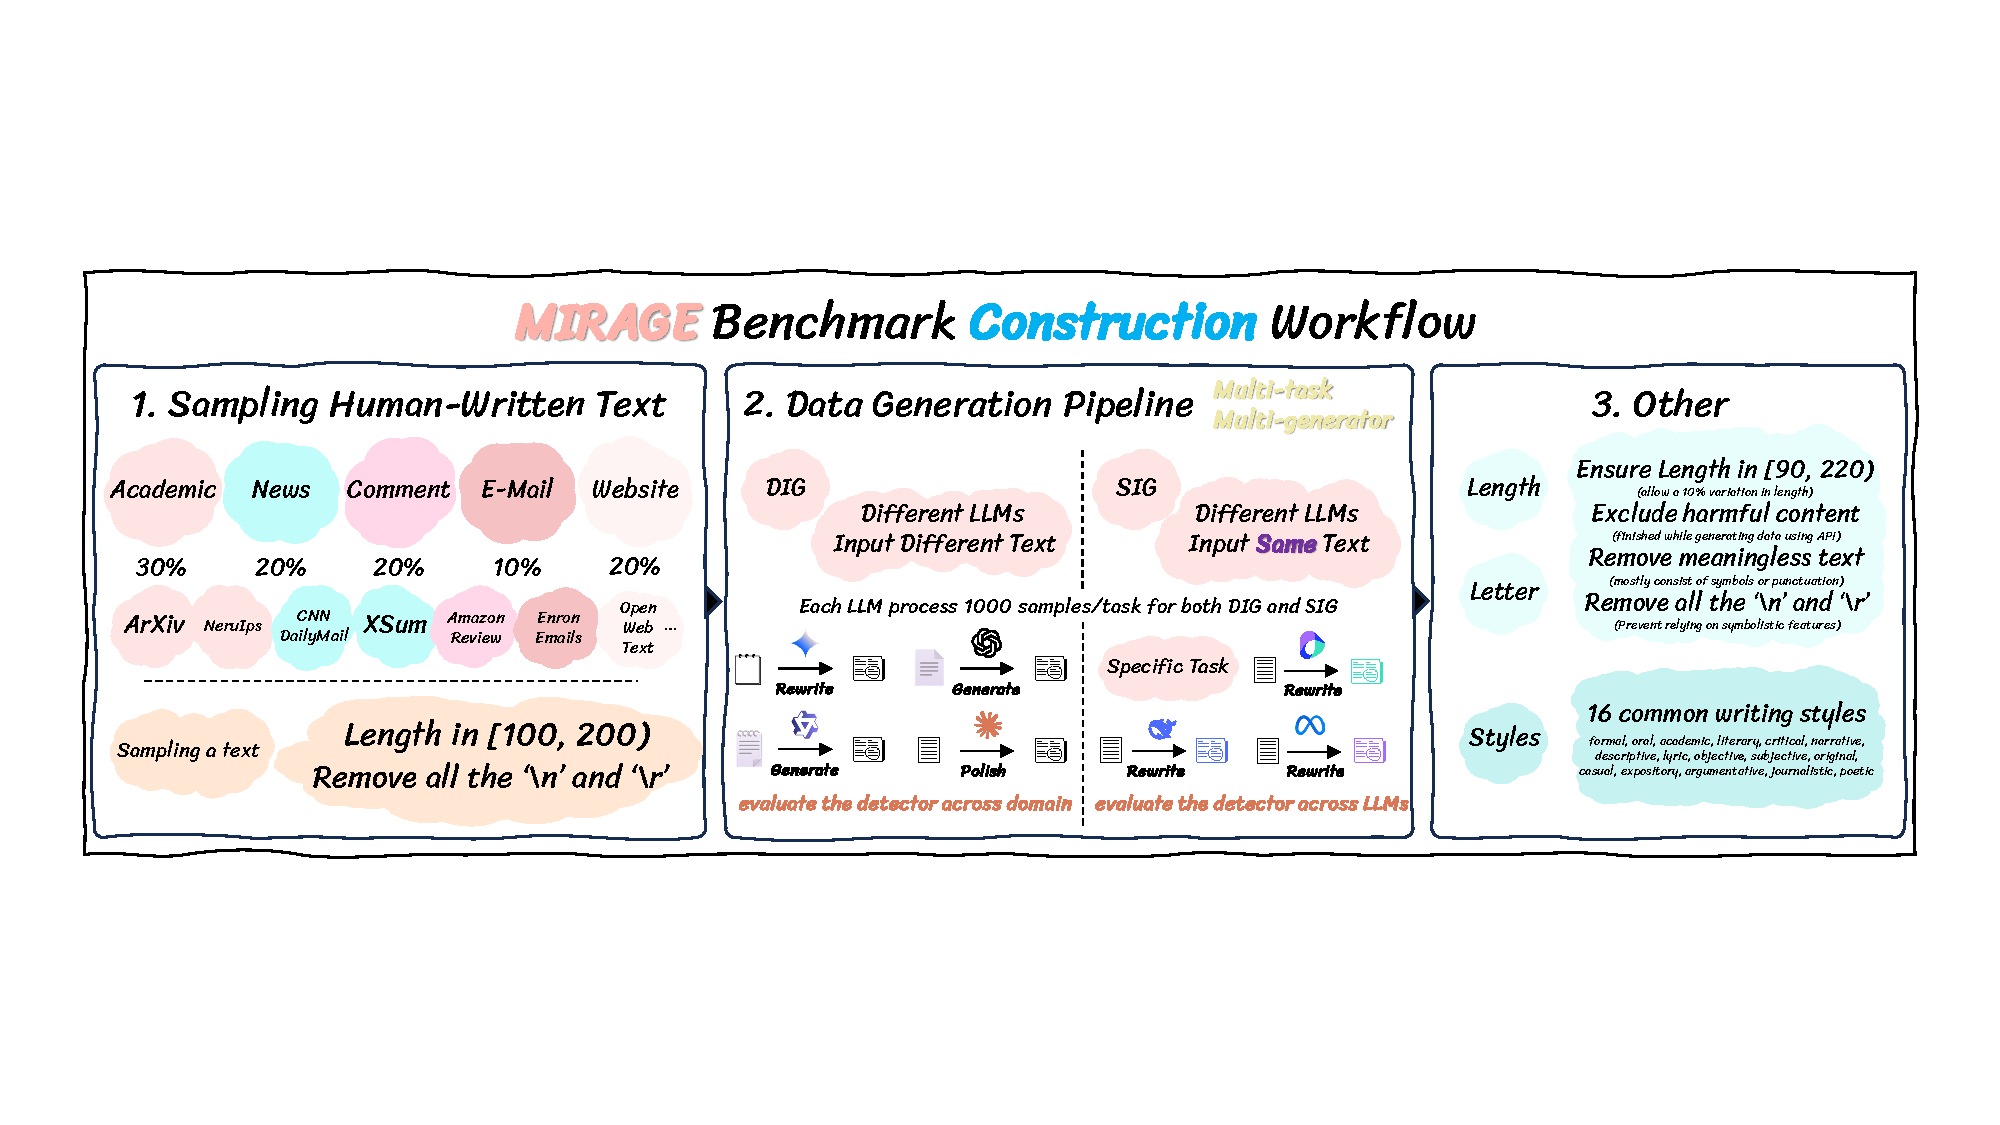
\includegraphics[width=\linewidth]{fig/workflow.pdf}
    \caption{The MIRAGE benchmark construction workflow. MIRAGE consists of 93K HWT-MGT pairs, significantly demonstrating diversity of text-domain, source LLM, and generation task, while using writing style control as augmentation. }
    \Description{Workflow of MIRAGE Benchmark.}
    \label{fig:workflow}
\end{figure*}
\section{Proposed MIRAGE Benchmark}
% Despite significant advancement in MGTD research in recent years, existing benchmarks still exhibit notable limitations in terms of Domain-Diversity and Source-LLMs Coverage.
% %
% The narrow range of text domains fails to reflect the diverse contexts in which LLMs are applied~\cite{turingbench, detectrl}, while the heavy reliance on small-scale, open-source models~\cite{m4bench, raid} neglects the widespread adoption of commercial, closed-source LLMs in practical applications.
% %
% Moreover, most existing benchmark datasets focus primarily on sampling for MGT while lacking consideration for MRT~\cite{mage, hc3}, which diverges from real-world scenarios.
% %
% These limitations hinder a thorough evaluation of current detection methods, resulting in models that perform well on specific datasets but struggle in broader, real-world applications.

% Current benchmarks often focus on narrow text domains~\cite{turingbench, detectrl} and primarily rely on small-scale, open-source models~\cite{m4bench, raid}, overlooking the prevalent use of commercial, closed-source LLMs in real-world applications. Furthermore, existing datasets predominantly emphasize MGT sampling while neglecting MRT~\cite{mage, hc3}, which misaligns with practical scenarios. 

Current benchmarks exhibit notable limitations in diversity of text domains~\cite{turingbench, detectrl}, coverage of source LLMs~\cite{m4bench, raid} and evaluation tasks~\cite{mage, hc3}.
%
These constraints hinder comprehensive assessment and lead to detection models with poor generalizability beyond narrowly defined benchmark scenarios.

In order to facilitate a robust evaluation that better reflect real-world application, we present the \textit{\textbf{M}ulti-domain \textbf{I}nclusive \textbf{R}ealistic \textbf{A}ssessment for machine \textbf{G}enerated text d\textbf{E}tection (\textbf{MIRAGE})} benchmark.
%
MIRAGE constitutes the most comprehensive multi-task MGTD evaluation framework to date, incorporating both generative and revisionary text across diverse domains, employing most advanced LLMs, including 13 proprietary and 4 open-source LLMs.


\subsection{Benchmark Construction}
 
\noindent \textbf{Multi-domain Sampling. }
Considering that LLMs exhibit varying performance across different text domains, MIRAGE sample HWT of 5 domains from 10 corpora, detail information are presented in Supplementary Material.

\noindent \textbf{Inclusive MGT Tasks. }
Following established methodologies in the ~\cite{fastdetectgpt} and ~\cite{imbd}, we designed three distinct MGT tasks: \textit{Generate}, \textit{Polish}, and \textit{Rewrite}.
%
The \textit{Generate} task involves creating new text based on the first 30 tokens of an HWT.
%
The \textit{Polish} task refines an existing HWT while preserving its original details and meaning.
%
The \textit{Rewrite} task paraphrases a given HWT without altering its meaning or essential details.
%
The detailed prompt of each task will be present in Supplementary Material.

\noindent \textbf{Realistic LLM Usage. }
In real-world scenarios, people typically rely on powerful commercial closed-source LLMs to generate or revise text.
%
However, most of existing benchmarks~\cite{turingbench, hc3, m4bench, mage, raid, detectrl} rely on open-source LLMs to create data, resulting in a gap between current benchmarks and real-world evaluations.
%
To address this, MIRAGE incorporates 13 mainstream commercial LLMs, as detailed in Supplementary Material.

Concurrently, recognizing the increasing deployment of high-performance open-source models in localized applications, we incorporated four advanced open-source LLMs~\cite{qwen2.5, llama3}, ensuring comprehensive coverage of the contemporary LLM ecosystem.

\noindent \textbf{Data Cleaning. }
We remove the `\textbackslash n' character from each data entry to prevent the detector from identifying MGT based on the presence of the `\textbackslash n' symbol. 
%
Subsequently, we segment the text into words using spaces and filter out texts containing 100-200 words from these datasets to control for length-based detection biases.

\noindent \textbf{Composition. }
We consider two distinct evaluation scenarios to reflect real-world applications:

\textit{\textbf{Disjoint-Input Generation(DIG):}} This assesses a detector's ability to distinguish between an original HWT and a corresponding MGT or MRT produced by a single LLM.

\textit{\textbf{Shared-Input Generation (SIG):}} This assesses a detector's capacity to simultaneously differentiate multiple MGTs or MRTs (produced by different LLMs) from the same original HWT.

%
We design each LLM to generate 2,000 samples for each MGT task, equally distributed between DIG and SIG scenarios (1,000 samples each).
%
To ensure the balance of text fields, both DIG and SIG maintained identical domain distribution ratios, as detailed in Supplementary Material.

Sampling begins with constructing domain level HWT datasets by proportionally merging source datasets within each domain.
%
Such dataset-mixing strategy ease dataset-bias by preventing oversampling from single dataset.

During implementation, SIG is treated as an independent ``model'' and incorporates alongside the 17 individual LLMs in the sampling process.
%
For each model (including SIG), we sequentially sample data from each domain dataset.
%
Once sampled, items are removed from corresponding domain datasets to maintain the distinction between DIG and SIG data.
%
Within each text domain, data is sampled continuously until the number of samples for that domain meets the requirements specified in Supplementary Material.
%
Once the data sampling for one text domain is complete, the process moves to the next, repeating until all text domains have been sampled.

This methodology produces the DIG dataset for each LLM and a comprehensive SIG dataset, which are subsequently combined to form the complete sample set for each LLM across all tasks.

\noindent \textbf{Data Augmentation. }
The language style is a key distinguishing feature between HWT and MGT, with a closer alignment to human language style posing a more challenging task for MGT detectors.
%
With this consideration, we introduce data augmentation in terms of LLM's language styles. 
%
Specifically, we incorporated the phrase ``in a <style> style" into the input prompt.
%
We manually select 16 different language styles, randomly choosing one during each LLM inference to achieve style-diversity.

This approach helps assess the robustness of detectors against content with varying language styles.
%
Moreover, in practice, one often adds language style constraints to prompts when using LLMs to assist with writing.
%
Thus, It further enhances the benchmark’s ability to simulate real-world scenarios.

\noindent \textbf{Post Cleaning. }
After generating MGT or MRT from the above HWT data, we perform data cleaning on the generated data.
%
First, all instances of the `\textbackslash n' and `\textbackslash r' are removed, to prevent detection from symbol's feature.
%
Next, we remove texts with fewer than 90 words or more than 220 words, to prevent the impact of text length variations on detection, and finally obtain the MIRAGE benchmark dataset.
%
The statistical results are presented in Supplementary Material.

\subsection{Evaluate Metrics}
Consistent with prior works~\cite{detectgpt, fastdetectgpt, imbd}, we adopt the \textit{Area Under the Receiver Operating Characteristic Curve (AUROC)} as the primary evaluation metric.
%
To assess the performance on specific threshold, we incorporate \textit{TPR at a 5\% false positive rate (TPR@5\%)} as a supplementary metric.
%
Furthermore, considering the MIRAGE-SIG is a class-imbalanced dataset, we additionally report the \textit{Matthews Correlation Coefficient (MCC)} and \textit{Balanced Accuracy} to provide a more comprehensive evaluation.
%
Together, this diverse set of metrics provides a comprehensive assessment of detector's performance, ensuring that the evaluation reflects both theoretical completeness and real-world applicability.
%
For more information on metrics, please see Supplementary Material.
\begin{table*}[htbp]
    \centering
    \caption{Results across three tasks (Generate, Polish, Rewrite) under two evaluation settings (MIRAGE-DIG and MIRAGE-SIG). All methods, except for RoBERTa-Base/Large, employ GPT-Neo-2.7B~\cite{gpt-neo} as the scoring model. Following with the experiment settings of~\cite{imbd}, the NPR~\cite{lrrandnpr} and DetectGPT~\cite{detectgpt} use T5-3B~\cite{t5} to generate perturbations, while Fast-DetectGPT~\cite{fastdetectgpt} utilizes GPT-J-6B~\cite{gpt-j} to generate samples. $\spadesuit$ indicates a training-based method, whereas $\diamondsuit$ denotes a method that requires multiple model invocations. "Imp." represents Improvement over previous SOTA, computed as $(new - old) / (1.0 - old)$. Metrics: AUROC, Balanced Accuracy, MCC, and TPR@5\%. DetectAnyLLM significantly outperforms all baselines across all tasks and settings.}
    \resizebox{\linewidth}{!}{
    \begin{tabular}{l|cccc|cccc|cccc}
    \hline

    \hline

    \hline
    \multicolumn{13}{c}{\textbf{MIRAGE-DIG (Disjoint-Input Generation)}}\\
    \hline

    \hline

    \hline
    \multirow{2}{*}{Methods}&\multicolumn{4}{c|}{Generate}&\multicolumn{4}{c|}{Polish}&\multicolumn{4}{c}{Rewrite} \\
    &  AUROC  &  Accuracy  &  MCC  &  TPR@5\%  &  AUROC  &  Accuracy  &  MCC  &  TPR@5\%  &  AUROC  &  Accuracy  &  MCC  &  TPR@5\%  \\
    \hline

    \hline
    Likelihood~\cite{likelihood} & 0.4936 & 0.5091 & 0.0183 & 0.0147 & 0.4653 & 0.5000 & 0.0000 & 0.0214 & 0.4337 & 0.5000 & 0.0000 & 0.0148 \\
    LogRank~\cite{logrank} & 0.4992 & 0.5128 & 0.0260 & 0.0220 & 0.4512 & 0.5000 & 0.0000 & 0.0195 & 0.4225 & 0.5000 & 0.0000 & 0.0132 \\
    Entropy~\cite{entropy} & 0.6522 & 0.6150 & 0.2543 & 0.1099 & 0.5543 & 0.5417 & 0.1247 & 0.0954 & 0.5805 & 0.5566 & 0.1650 & 0.1189 \\
    RoBERTa-Base~\cite{roberta} $\spadesuit$ & 0.5523 & 0.5397 & 0.1434 & 0.1250 & 0.4859 & 0.5010 & 0.0088 & 0.0460 & 0.5020 & 0.5049 & 0.0293 & 0.0569 \\
    RoBERTa-Large~\cite{roberta} $\spadesuit$ & 0.4716 & 0.5217 & 0.0842 & 0.0871 & 0.5171 & 0.5151 & 0.0340 & 0.0633 & 0.5570 & 0.5385 & 0.0864 & 0.0895 \\
    LRR~\cite{lrrandnpr} & 0.5215 & 0.5341 & 0.0777 & 0.0701 & 0.4081 & 0.5000 & 0.0000 & 0.0200 & 0.3930 & 0.5000 & 0.0000 & 0.0188 \\
    DNA-GPT~\cite{dna-gpt} $\diamondsuit$ & 0.5733 & 0.5595 & 0.1196 & 0.0776 & 0.4771 & 0.5004 & 0.0110 & 0.0309 & 0.4453 & 0.5001 & 0.0080 & 0.0251 \\
    NPR~\cite{lrrandnpr} $\diamondsuit$ & 0.6120 & 0.6140 & 0.2604 & 0.0191 & 0.5071 & 0.5370 & 0.1071 & 0.0318 & 0.4710 & 0.5201 & 0.0663 & 0.0226 \\
    DetectGPT~\cite{detectgpt} $\diamondsuit$ & 0.6402 & 0.6258 & 0.2758 & 0.0275 & 0.5469 & 0.5531 & 0.1328 & 0.0355 & 0.5061 & 0.5266 & 0.0826 & 0.0283 \\
    Fast-DetectGPT~\cite{fastdetectgpt} & 0.7768 & 0.7234 & 0.4628 & 0.4310 & 0.5720 & 0.5570 & 0.1293 & 0.1189 & 0.5455 & 0.5432 & 0.1015 & 0.1025 \\
    ImBD~\cite{imbd} $\spadesuit$ & 0.8597 & 0.7738 & 0.5497 & 0.4065 & 0.7888 & 0.7148 & 0.4300 & 0.2730 & 0.7825 & 0.7068 & 0.4139 & 0.2933 \\
    \hdashline
    
    \hdashline
    \rowcolor[HTML]{fff5f4}
    
    \textbf{DetectAnyLLM} (ours) $\spadesuit$ & \textbf{0.9525} & \textbf{0.8988} & \textbf{0.7975} & \textbf{0.7770} & \textbf{0.9297} & \textbf{0.8732} & \textbf{0.7487} & \textbf{0.7756} & \textbf{0.9234} & \textbf{0.8705} & \textbf{0.7447} & \textbf{0.7778} \\
    
    \rowcolor[HTML]{fff5f4}
    
    \textbf{Imp.} & \red{+66.14\%} & \red{+55.26\%} & \red{+55.03\%} & \red{+62.43\%} & \red{+66.71\%} & \red{+55.54\%} & \red{+55.91\%} & \red{+69.13\%} & \red{+64.78\%} & \red{+55.83\%} & \red{+56.44\%} & \red{+68.56\%} \\
    \hline

    \hline

    \hline
    \multicolumn{13}{c}{\textbf{MIRAGE-SIG (Shared-Input Generation)}}\\
    \hline

    \hline

    \hline
    \multirow{2}{*}{Methods}&\multicolumn{4}{c|}{Generate}&\multicolumn{4}{c|}{Polish}&\multicolumn{4}{c}{Rewrite} \\
    &  AUROC  &  Accuracy  &  MCC  &  TPR@5\%  &  AUROC  &  Accuracy  &  MCC  &  TPR@5\%  &  AUROC  &  Accuracy  &  MCC  &  TPR@5\%  \\
    \hline

    \hline
    Likelihood~\cite{likelihood} & 0.4968 & 0.5207 & 0.0196 & 0.0145 & 0.4599 & 0.5002 & 0.0030 & 0.0233 & 0.4319 & 0.5000 & 0.0000 & 0.0111 \\
    LogRank~\cite{logrank} & 0.5008 & 0.5183 & 0.0182 & 0.0186 & 0.4468 & 0.5000 & 0.0000 & 0.0211 & 0.4221 & 0.5000 & 0.0000 & 0.0118 \\  
    Entropy~\cite{entropy} & 0.6442 & 0.6123 & 0.1592 & 0.1074 & 0.5640 & 0.5439 & 0.0516 & 0.0946 & 0.5858 & 0.5645 & 0.0918 & 0.1198 \\  
    RoBERTa-Base~\cite{roberta} $\spadesuit$ & 0.5368 & 0.5392 & 0.0529 & 0.1101 & 0.4741 & 0.5011 & 0.0048 & 0.0395 & 0.5099 & 0.5122 & 0.0221 & 0.0668 \\
    RoBERTa-Large~\cite{roberta} $\spadesuit$ & 0.4703 & 0.5236 & 0.0417 & 0.0910 & 0.5150 & 0.5157 & 0.0283 & 0.0702 & 0.5576 & 0.5426 & 0.0405 & 0.0762 \\
    LRR~\cite{lrrandnpr} & 0.5214 & 0.5311 & 0.0314 & 0.0657 & 0.4076 & 0.5000 & 0.0000 & 0.0238 & 0.3978 & 0.5000 & 0.0000 & 0.0174 \\    
    DNA-GPT~\cite{dna-gpt} $\diamondsuit$ & 0.5759 & 0.5647 & 0.0603 & 0.0813 & 0.4788 & 0.5001 & 0.0036 & 0.0340 & 0.4457 & 0.5002 & 0.0048 & 0.0258 \\
    NPR~\cite{lrrandnpr} $\diamondsuit$ & 0.6088 & 0.6170 & 0.1571 & 0.0185 & 0.5074 & 0.5277 & 0.0612 & 0.0293 & 0.4738 & 0.5204 & 0.0340 & 0.0177 \\
    DetectGPT~\cite{detectgpt} $\diamondsuit$ & 0.6353 & 0.6241 & 0.1719 & 0.0193 & 0.5434 & 0.5515 & 0.0668 & 0.0309 & 0.5079 & 0.5260 & 0.0431 & 0.0239 \\
    Fast-DetectGPT~\cite{fastdetectgpt} & 0.7706 & 0.7193 & 0.2078 & 0.4200 & 0.5727 & 0.5619 & 0.0607 & 0.1238 & 0.5480 & 0.5495 & 0.0525 & 0.1097 \\
    ImBD~\cite{imbd} $\spadesuit$ & 0.8612 & 0.7791 & 0.5599 & 0.4183 & 0.7951 & 0.7199 & 0.4451 & 0.3036 & 0.7694 & 0.6920 & 0.3936 & 0.2868 \\
    \hdashline
    
    \hdashline
    \rowcolor[HTML]{fff5f4}
    \textbf{DetectAnyLLM} (ours) $\spadesuit$ & \textbf{0.9526} & \textbf{0.9059} & \textbf{0.8119} & \textbf{0.7722} & \textbf{0.9316} & \textbf{0.8740} & \textbf{0.7483} & \textbf{0.7779} & \textbf{0.9158} & \textbf{0.8643} & \textbf{0.7320} & \textbf{0.7574} \\
    
    \rowcolor[HTML]{fff5f4}
    \textbf{Imp.} & \red{+65.85\%} & \red{+57.40\%} & \red{+57.25\%} & \red{+60.84\%} & \red{+66.62\%} & \red{+55.02\%} & \red{+54.64\%} & \red{+68.11\%} & \red{+63.49\%} & \red{+55.94\%} & \red{+55.80\%} & \red{+65.98\%} \\
    \hline

    \hline

    \hline
    \end{tabular}
    }
    
    \label{tab:main_results}
\end{table*}
\section{Experiment}
\subsection{Main Results}\label{main_result}
% We evaluate \textit{DetectAnyLLM} against a broad range of strong baselines across two challenging subsets---\textbf{MIRAGE-DIG} and \textbf{MIRAGE-SIG}.
% %
% Across all three MGTD tasks (Generate, Polish, Rewrite), our method consistently achieves the highest scores in all metrics, including AUROC, Accuracy, MCC, and TPR@5\%.

\noindent \textbf{Training settings. }
To achieve a fair comparison, the scoring model used in DetectAnyLLM is the same as ~\cite{imbd}(i.e., GPT-Neo-2.7B~\cite{gpt-neo}).
%
Additionally, we adopt the same training dataset as~\cite{imbd} to maintain consistency.
%
Further training settings are provided in the Supplementary Material.
%on hyperparameters such as learning rate and number of training epochs 
We set the $\gamma$ in DDL's training objective to 100, and will further discuss how $\gamma$ affects the detector's performance in \Cref{ablation_study}.

\noindent \textbf{Baselines. }
For a comprehensive comparison, we compare the performance of our method with classical methods, advanced zero-shot methods, and state-of-the-art training-based methods.
%
The classical methods including \textit{Likelihood}~\cite{likelihood}, \textit{Log-Rank}~\cite{logrank}, \textit{LRR}~\cite{lrrandnpr}, and \textit{Entropy}~\cite{entropy}.
%
The advanced zero-shot methods includes \textit{DetectGPT}~\cite{detectgpt}, \textit{NPR}~\cite{lrrandnpr}, and \textit{Fast-DetectGPT}~\cite{fastdetectgpt}.
%
The training-based methods includes \textit{RoBERTa series}~\cite{roberta, likelihood} and \textit{ImBD}~\cite{imbd}.

\noindent \textbf{Results of MIRAGE-DIG. }
As the top of \Cref{tab:main_results} shown, DetectAnyLLM achieves substantial performance improvement over all baselines across all metrics and tasks.
%
Specifically, it delivers AUROC gains of up to \red{+63.49\%}$\sim$ \red{+66.71\%}, with MCC improvements reaching up to \red{+57.25\%}.
%
DetectAnyLLM also maintains robust TPR@5\% across all tasks, outperforming previous training-based SOTA ImBD~\cite{imbd} by large margins (\red{+60.84\%}$\sim$ \red{+69.13\%}).

\noindent \textbf{Results of MIRAGE-SIG. }
As the bottom of \Cref{tab:main_results} shown, DetectAnyLLM continues to lead under the more challenging MIRAGE-SIG setting, reaching AUROC of \red{0.9526}, Balanced Accuracy of \red{0.9059}, and TPR@5\% up to \red{0.7779}, again greatly surpassing all other methods. 
%
Notably, even in the Rewrite task—--where performance is generally lower across all models--—DetectAnyLLM maintains high robustness (AUROC: \red{0.9158}, TPR@5\%: \red{0.7574}).
%
The results highlight the detector’s strong generalization capability across diverse source LLMs, even when these LLMs generate or revise the same underlying text, demonstrating the robustness of our method in real-world applications.

\begin{table}[htbp]
    \centering
    \caption{Results of detection on the previous test sets. $\spadesuit$ indicates a training-based method, whereas $\diamondsuit$ denotes a method that requires multiple model invocations. "Imp." represents Improvement, computed as $(new - old) / (1.0 - old)$.}
    \resizebox{\linewidth}{!}{
    \begin{tabular}{l|ccc}
    \hline

    \hline

    \hline
    \multicolumn{4}{c}{\textbf{ImBD~\cite{imbd} Test Dataset (GPT-4o polished)}}\\
    \hline

    \hline

    \hline
    Methods&XSum~\cite{xsum}&Writing~\cite{writting_prompts} & PubMed~\cite{pubmedqa}\\
    \hline

    \hline
    Likelihood~\cite{likelihood} & 0.4396 & 0.8077 & 0.4596\\
    LogRank~\cite{logrank} & 0.4002 & 0.7694 & 0.4472\\
    Entropy~\cite{entropy} & 0.6122 & 0.2802 & 0.5899\\
    RoBERTa-Base~\cite{roberta} $\spadesuit$ & 0.4921 & 0.4774 & 0.2496 \\
    RoBERTa-Large~\cite{roberta} $\spadesuit$ & 0.4782 & 0.4708 & 0.3089 \\
    LRR~\cite{lrrandnpr} & 0.3095 & 0.6214 & 0.4710 \\
    DNA-GPT~\cite{dna-gpt} $\diamondsuit$ & 0.4974 & 0.7478 & 0.3151 \\
    NPR~\cite{lrrandnpr} $\diamondsuit$ & 0.5065 & 0.8444 & 0.3740 \\
    DetectGPT~\cite{detectgpt} $\diamondsuit$ & 0.6217 & 0.8771 & 0.5612\\
    Fast-DetectGPT~\cite{fastdetectgpt} & 0.6293 & 0.8324 & 0.6175\\
    ImBD~\cite{imbd} $\spadesuit$ & 0.9486 & 0.9468 & 0.7743\\
    \hdashline
    
    \hdashline
    \rowcolor[HTML]{fff5f4}
    \textbf{DetectAnyLLM} (ours) $\spadesuit$ & \textbf{0.9880} & \textbf{0.9671} & \textbf{0.8817} \\
    
    \rowcolor[HTML]{fff5f4}
    \textbf{Imp.} & \red{+80.16\%} & \red{+38.16\%} & \red{+47.59\%} \\
    \hline

    \hline

    \hline
    \end{tabular}
    }
    
    \label{tab:previous_dataset}
\end{table}

\noindent \textbf{Detection on the previous test sets. }
We evaluate the performance of DetectAnyLLM on the three test sets used by ImBD~\cite{imbd}, comprising 150 texts sampled from XSum~\cite{xsum}, WritingPrompts~\cite{writting_prompts}, and PubMedQA~\cite{pubmedqa}, respectively, each polished by GPT-4o.
%
As ~\Cref{tab:previous_dataset} shown, DetectAnyLLM consistently outperforms all existing MGTD methods.

However, while prior methods perform reasonably well on these test sets, their performance degraded greatly on MIRAGE, as ~\Cref{tab:main_results} shown.
%
This observation reveals the limitations of existing benchmarks in fully capturing detector capabilities and further underscores the importance of MIRAGE as a more challenging and comprehensive benchmark for evaluating detection robustness.

\noindent \textbf{Efficiency comparison. }
Since DDL performs optimization without relying on a reference model, it achieves substantial improvements in training efficiency compared to \textit{Style Preference Optimization (SPO)}~\cite{imbd}.
%
DDL demonstrates a \red{+30.12\%} reduction in training time and a \red{+35.90\%} reduction in memory consumption relative to SPO~\cite{imbd}.
%
Detailed results are provided in Supplementary Material.


\subsection{Ablation Study}\label{ablation_study}
\noindent \textbf{Ablation on parameter $\gamma$. }
As shown in ~\Cref{tab:ablation_gamma}, DDL exhibits strong robustness for the values of $\gamma$.
% 
Compared to the results in ~\Cref{tab:main_results}, for all selected values of $\gamma$, the trained detector consistently outperforms all prior state-of-the-art methods in terms of AUROC.
%
We provide detail results and further perform comprehensive analysis and discussion later in Supplementary Material.

\begin{table}[htbp]
    \centering
    \caption{Results of different $\gamma$ in DDL. Metrics with subscript $_t$ correspond to the training set, and subscript $_v$ indicates evaluation on the polish task of MIRAGE-DIG.}
    \resizebox{\linewidth}{!}{
    \begin{tabular}{l|cccccc}
    \hline

    \hline

    \hline
    & $\gamma=10$  & $\gamma=20$ & $\gamma = 50$  & $\gamma=100$  & $\gamma=500$ & $\gamma=10000$\\
    \hline
    AUROC$_t$  &  \textbf{0.9964} & 0.9934 & 0.9883 & 0.9861 & 0.9861 & 0.9861\\
    AUPR$_t$   &  \textbf{0.9965} & 0.9938 & 0.9888 & 0.9833 & 0.9833 & 0.9833\\
    \hdashline
    \rowcolor[HTML]{fff5f4}
    AUROC$_v$  & 0.8692  & 0.9257 & \textbf{0.9347} & 0.9259 & 0.9259 & 0.9259\\
    \rowcolor[HTML]{fff5f4}
    AUPR$_v$   & 0.8735  & 0.9294 & \textbf{0.9458} & 0.9373 & 0.9373 & 0.9373\\
    \hline

    \hline

    \hline
    \end{tabular}
    }
    \label{tab:ablation_gamma}
\end{table}

\noindent \textbf{Ablation on KL-strength $\beta$ in SPO~\cite{imbd}. } We provide comprehensive experiments and confirm our point in~\Cref{redundant KL-regularization}.
%
For more information, please see Supplementary Material.

\noindent \textbf{Ablation on model size. }
We retrain Qwen2-0.5B~\cite{qwen2}, GPT-Neo-2.7B~\cite{gpt-neo}, and GPT-J-6B~\cite{gpt-j} using SPO~\cite{imbd} and DDL, while keeping the training data and optimization settings fixed.
%
The models are then evaluated on the \textit{Polish} task of MIRAGE-DIG.

As~\Cref{tab:ablation_model_size} shown, the DDL-optimized detector consistently outperforms the SPO~\cite{imbd}-optimized ones across all model sizes, confirming DDL's robustness and adaptability.
%
Notably, DDL achieves strong performance even with small models, such as Qwen2-0.5B~\cite{qwen2}, and scales effectively with larger backbones.
%
This result highlights the effectiveness of DDL in fully leveraging model capacity.

\begin{table}[htbp]
    \centering
    \caption{Ablation study on the impact of scoring model size. All models are trained on the same data and evaluated on the MIRAGE-SIG \textit{Rewrite} task. Improvement is marked \red{red}.}
    \resizebox{\linewidth}{!}{
    \begin{tabular}{c|lcccc}
    \hline

    \hline

    \hline
    Method & Base Model &  AUROC  &  Accuracy  &  MCC & TPR@5\%\\
    \hline
    \multirow{3}{*}{SPO~\cite{imbd}}&Qwen2-0.5B~\cite{qwen2} & 0.8570 & 0.7816 & 0.5632 & 0.4508\\
    &GPT-Neo-2.7B~\cite{gpt-neo}& 0.7694 & 0.6920 & 0.3936 & 0.2868\\
    &GPT-J-6B~\cite{gpt-j}& 0.8367 & 0.7557 & 0.5155 & 0.4722\\
    \hline
    \multirow{6}{*}{DDL (ours)}&\multirow{2}{*}{Qwen2-0.5B~\cite{qwen2}} & 0.9370 & 0.9071 & 0.8169 & 0.8575\\
    && \red{+55.94\%} & \red{+57.46\%} & \red{+58.08\%} & \red{+74.05\%}\\
    \cdashline{2-6}
    &\multirow{2}{*}{GPT-Neo-2.7B~\cite{gpt-neo}}& 0.9158 & 0.8643 & 0.7320 & 0.7574\\
    && \red{+63.49\%} & \red{+55.94\%} & \red{+55.80\%} & \red{+65.98\%}\\
    \cdashline{2-6}
    &\multirow{2}{*}{GPT-J-6B~\cite{gpt-j}}& 0.8909 & 0.8424 & 0.6878 & 0.6047\\
    && \red{+33.19\%} & \red{+35.49\%} & \red{+35.56\%} & \red{+25.10\%}\\
    \hline

    \hline

    \hline
    \end{tabular}
    }
    \label{tab:ablation_model_size}
\end{table}

\noindent \textbf{Ablation on normalization $\sigma$. }\label{ablation_on_sigma}
% Since DDL optimizes the scoring model by directly learning discrepancy, the normalization term $\sigma$ plays a critical role during training.
%
% To assess the impact of normalization item $\sigma$ in discrepancy, we conduct an ablation study using DDL to optimize the same scoring model with and without the inclusion of the normalization term $\sigma$ in the objective.
As shown in~\Cref{tab:ablation_normalization}, the removal of $\sigma$ leads to a substantial degradation in performance across all metrics, highlighting the importance of $\sigma$ for stable and effective optimization.
%
Despite this, DDL without normalization still surpasses previous state-of-the-art methods on most metrics reported in~\Cref{tab:main_results}, underscoring the robustness of DDL.
%
We suggest that the normalization item $\sigma$ helps standardize output across diverse source LLMs and domains, thereby facilitating more consistent and generalizable learning.

\begin{table}[htbp]
    \centering
    \caption{Ablated result of $\sigma$. ``norm.'' means ``normalization''. ``w/'' means ``with'' and ``w/o'' means ``without''. Scoring model: GPT-Neo-2.7B~\cite{gpt-neo}. Benchmark: MIRAGE-DIG-polish.}
    \begin{tabular}{l|cccc}
    \hline

    \hline

    \hline
         &  AUROC  &  Accuracy  &  MCC & TPR@5\%\\
    \hline
    DDL$_{\textbf{w/o}\enspace norm.}$ & 0.6923 & 0.6604 & 0.3244 & 0.0999\\
    \hdashline
    \rowcolor[HTML]{fff5f4}
    DDL$_{\textbf{w/}\enspace norm.}$& \textbf{0.9261} & \textbf{0.8691} & \textbf{0.7399} & \textbf{0.7615}\\
    \hline

    \hline

    \hline
    \end{tabular}
    \label{tab:ablation_normalization}
\end{table}
\section{Conclusion}
In this study, we have introduced a novel optimization strategy, \textit{Direct Discrepancy Learning (DDL)}, and developed a unified detection framework named \textit{DetectAnyLLM}.
%
Our approach enables the scoring model to acquire task-oriented knowledge by directly leveraging discrepancy signals and achieves high-precision detection through a technique we call \textit{reference clustering}.
%
We also proposed \textit{MIRAGE}, a comprehensive benchmark dataset that spans a wide range of text domains, the most advanced LLMs, and generation tasks.
%
To thoroughly evaluate detector performance, we assessed DetectAnyLLM and existing MGTD methods under two settings: \textit{Disjoint-Input Generation} and \textit{Shared-Input Generation}.
%
Experimental results on both MIRAGE and previously established test sets demonstrate that DetectAnyLLM significantly outperforms existing MGTD methods, establishing a new state-of-the-art in this domain.

\clearpage
\bibliographystyle{sec/ACM-Reference-Format}
\bibliography{sec/ref}
\end{document}
\endinput
%%
%% End of file `sample-sigconf-authordraft.tex'.
